\documentclass[tombow,dvipdfmx]{corona-a5-1.1}
% dvipdfmxを追加(川口)

% Springer document settings
\usepackage[bottom]{footmisc}% places footnotes at page bottom

\usepackage{newtxtext}       % 
\usepackage[varvw]{newtxmath}       % selects Times Roman as basic font
%%%%%%%%%%%%%%%%%%%%%%%%%%%%%%%

% \usepackage{amssymb}
\usepackage{ntheorem}
\usepackage{amsmath}
\usepackage{enumitem}


\usepackage{graphicx}
\usepackage{color}
\usepackage{cite}
\usepackage{makeidx}


\usepackage{ascmac}
\usepackage{eclbkbox}
\usepackage{dsfont}

\usepackage{longtable}

\usepackage{url}

\usepackage{hyperref}

\usepackage{multicol}

%% --川口追加--
\makeatletter
\let\MYcaption\@makecaption
\makeatother
\usepackage{subcaption}
\captionsetup{compatibility=false}      % 必要に応じて

\makeatletter
\let\@makecaption\MYcaption
\makeatother
% ----

%%
\theoremstyle{plain}
\theoremheaderfont{\bfseries}
\theorembodyfont{\rmfamily}
\theoremseparator{\hspace{1ex}}
\theoremindent0cm
\theoremnumbering{arabic}
\theoremprework{\vspace{1ex}\begin{shadebox}\vspace{1ex}}
\theorempostwork{\vspace{-1ex}\end{shadebox}\vspace{1ex}}

%%
\theoremclass{theorem}

%%
\theoremclass{theorem}

%%
\theoremclass{theorem}


%%
\theoremstyle{break}
\theoremheaderfont{\bfseries}
\theorembodyfont{\rmfamily}
\theoremseparator{}
\theoremindent0cm
\theoremnumbering{arabic}
\theoremprework{\vspace{1.5ex}\begin{breakbox}\vspace{-0.5ex}}
\theorempostwork{\vspace{-0.5ex}\end{breakbox}\vspace{1.5ex}}

%%
\theoremstyle{nonumberplain}
\theoremseparator{\hspace{1ex}}

%%
\newtheorem{assumption}{Assumption}[section]

%%
\renewcommand{\theproblem}{}

\renewcommand{\theremark}{}


\newcommand{\red}[1]{{\color{red}#1}}
\newcommand{\blue}[1]{{\color{blue}#1}}
\newcommand{\green}[1]{{\color{green}#1}}

\DeclareMathOperator*{\argmax}{arg\,max}

\newcommand{\bm}[1]{\boldsymbol{#1}}
\newcommand{\sfT}{\mathsf{T}}

\newcommand{\advanced}{$^{\ddag}$}

\DeclareMathOperator{\sfsin}{\mathsf{sin}}
\DeclareMathOperator{\sfcos}{\mathsf{cos}}
\DeclareMathOperator{\sftan}{\mathsf{tan}}
\DeclareMathOperator{\sfarctan}{\mathsf{arctan}}

\DeclareMathOperator{\sfdiag}{\mathsf{diag}}
\DeclareMathOperator{\sfcol}{\mathsf{col}}
\DeclareMathOperator{\sfdet}{\mathsf{det}}
\DeclareMathOperator{\sfadj}{\mathsf{adj}}
\DeclareMathOperator{\sftrace}{\mathsf{trace}}

\DeclareMathOperator{\real}{\mathsf{Re}}

\DeclareMathOperator{\sfker}{\mathsf{ker}}
\DeclareMathOperator{\sfim}{\mathsf{im}}

\DeclareMathOperator{\sfdim}{\mathsf{dim}}
\DeclareMathOperator{\sfspan}{\mathsf{span}}

\DeclareMathOperator{\sfint}{\mathsf{int}}

\DeclareMathOperator*{\sfmin}{\mathsf{min}}
\DeclareMathOperator*{\sfmax}{\mathsf{max}}
\DeclareMathOperator*{\sfsup}{\mathsf{sup}}

\DeclareMathOperator{\sfsat}{\mathsf{sat}}

\newcommand{\mat}[1]{\left[\: \begin{matrix} #1 \end{matrix} \:\right]}
\newcommand{\spliteq}[1]{\begin{split} #1 \end{split}}
\newcommand{\simode}[1]{\begin{cases}  \begin{split} #1 \end{split} \end{cases}}

\newcommand{\proofend}{\hfill \rule{2mm}{3mm}}

\newcommand{\Xti}{X_i'}
\newcommand{\Xsi}{X_i}

\newcommand{\Xtone}{X_1'}
\newcommand{\XtN}{X_N'}

\newcommand{\Xt}{X'}
\newcommand{\Xs}{X}

\newcommand{\taudi}{\tau_i}
\newcommand{\taud}{\tau}

\newcommand{\Cgi}{b_i}


\newcommand{\Ifd}{I_{\rm field} }

\newcommand{\matlab}{\textsc{Matlab} }





%% --川口追加--
\newcommand{\thshift}{\theta_{12}}
\newcommand{\thshiftb}{\theta_{32}}
\newcommand{\Ysa}{\bm y_{12}}
\newcommand{\bca}{c_{12}}
\newcommand{\Ysb}{\bm y_{32}}
\newcommand{\bcb}{c_{32}}
\newcommand{\bcij}{c_{ij}}
\newcommand{\Is}{{\bm I}_{12}' }
\newcommand{\im}{\bm j}
\newcommand{\tr}{{\sf T}}

%%%%%%%%%%%%%%%%%%%%%%%%% code lines %%%%%%%%%%%%%%%%%%%%%%%%%%%%%%%%%%%%%%%%%%
\usepackage{listings}
\usepackage{xcolor}
\renewcommand{\lstlistingname}{Program}% Listing -> Algorithm
\renewcommand{\lstlistlistingname}{List of \lstlistingname s}% List of Listings -> List of Algorithms

\definecolor{codegreen}{rgb}{0,0.6,0}
\definecolor{codegray}{rgb}{0.5,0.5,0.5}
\definecolor{codepurple}{rgb}{0.58,0,0.82}
\definecolor{backcolour}{rgb}{0.95,0.95,0.92}

\lstdefinestyle{mystyle}{
    backgroundcolor=\color{backcolour},   
    commentstyle=\color{codegreen},
    keywordstyle=\color{magenta},
    numberstyle=\tiny\color{codegray},
    stringstyle=\color{codepurple},
    basicstyle=\ttfamily\footnotesize,
    breakatwhitespace=false,         
    breaklines=true,                 
    captionpos=b,                    
    keepspaces=true,                 
    numbers=left,                    
    numbersep=5pt,                  
    showspaces=false,                
    showstringspaces=false,
    showtabs=false,                  
    tabsize=2
}

\lstset{style=mystyle}


\begin{document}
\newcommand{\omitcode}{~(省略)~}


\chapter{電力系統モデルの数値シミュレーション}\label{chap:numcal}

チャプター概要

\section{電力系統モデルの時間応答を計算するためには}\label{sec:howtocal}

\subsection{時間応答を計算することの難しさ}

\ref{ch:model}章では,微分方程式で表される発電機モデルや代数方程式で表される負荷モデルが,代数方程式で表される送電網モデルで結合されることにより,電力系統全体の数理モデルが非線形微分代数方程式の形式で記述されることを説明した。
したがって,電力系統モデルの時間応答は,適当に設定された初期値や外部入力のもとで,その微分代数方程式を数値積分することにより計算することができる。
しかしながら,電力系統モデルの数値シミュレーションでは,
\begin{itemize}
\item 外部入力を正しく設定しない限り需要と供給が均衡しないため,周波数偏差の定常値が0にならず,発電機の回転子偏角が変化し続ける
\item 周波数偏差の定常値が0となるような外部入力値の組み合わせは無数に存在するため,現実的に妥当な外部入力値を指定しなければならない
\item 母線群の電圧フェーザや電流フェーザの値は,発電機群の状態変数に対する従属変数として整合するように決定しなければならない
\end{itemize}
など,電力系統に特有の性質を十分に考慮する必要がある。
このため,MATLABに標準実装されている微分代数方程式ソルバーを単純に使用するだけでは,電力系統の数値シミュレーションを正しく実行することはできない。
この点が電力系統モデルの時間応答の計算を難しくする一因となる。

\subsection{計算手順}\label{sec:numstep}

電力系統モデルの時間応答の標準的な計算手順は,つぎの3ステップに分けられる。

\begin{itemize}
\item[(A)] 解析する需要と供給が均衡した電力系統状態を指定するため,送電網から定まるアドミタンス行列を用いて,定常状態におけるすべての母線の電流フェーザと電圧フェーザの値を計算する。
\item[(B)] 決定された母線の電流フェーザと電圧フェーザの定常値に整合するように,各発電機の内部電圧や回転子偏角の定常値,発電機への外部入力値,各負荷のインピーダンス値などを逆算する。
\item[(C)] ステップAとステップBで計算された需給が均衡した電力系統状態を初期値として,発電機の内部状態に外乱を与える,母線の電圧を地絡させる,負荷のパラメータ値を変化させる,などの大小様々な外乱を生じさせた場合の時間応答を計算する。
\end{itemize}

システム制御工学の観点では,ステップAは「無数に存在する平衡点の中から数値的な解析を行う平衡点を1つ定めること」と理解することができる。
\ref{sec:paradef}節で後述するように,すべての母線における電流フェーザと電圧フェーザの定常値が与えられたときに,それらを実現する発電機の内部状態の定常値や外部入力値,負荷のパラメータ値は必ず存在する。
このことから,すべての母線における電流フェーザと電圧フェーザの定常値を計算することは,微分代数方程式で表される電力系統モデルの平衡点を計算することに等しい。
電力系統工学では,このプロセスのことを\emph{潮流計算}(power flow calculation)と呼ぶ。
なお,各母線の電流フェーザと電圧フェーザの定常値を求めることは,各機器から母線に供給される有効電力と無効電力の定常値を求めることと数学的に等価である。

ステップBでは,母線の電流フェーザや電圧フェーザの定常値に整合するように発電機の内部状態の定常値や外部入力値,負荷のパラメータ値を逆算する。
このステップで注意が必要なのは,負荷のパラメータ値,すなわち,負荷の数理モデルは,「ステップAの潮流計算の結果から逆算されて定められる」という点である。
例えば,ある母線に接続する負荷を定インピーダンスモデルに設定したい場合には,潮流計算で求められた母線の電流フェーザを電流フェーザで除した値として,負荷のインピーダンス値を逆算するという手順を踏む。
負荷モデルのパラメータを所望の値に設定したい場合には,ステップCにおいて,負荷のパラメータ変動に対する時間応答を計算しながら,負荷のパラメータ値を所望の値に変化させるなどの方法を用いる。


さいごに,ステップCでは,目的に応じた様々な条件で電力系統モデルの時間応答を計算する。
例えば,ステップAとBで計算された各発電機への外部入力値や負荷のパラメータ値を定数としてモデルに設定し,発電機の内部状態に適当な初期値を与えて時間応答を計算すれば,時間の経過にしたがって,発電機の内部状態はステップBで計算された定常状態に漸近的に収束する。
ただし,漸近収束が成り立つような妥当な初期値を設定するためには,ステップAとBのように,解析の基準となる平衡点をあらかじめ計算しておく必要がある。
また,計算された平衡点は適切な意味で安定でなければならない。


\section{定常状態を数値的に探索する潮流計算}\label{sec:powflow}

本節では,\ref{sec:numstep}節のステップAとして説明された,電力系統の定常状態を数値的に探索する潮流計算の概要やMATLABによる実装方法を述べる。
以下では,与えられたアドミタンス行列$\bm{Y}$に対して,
 \begin{align}\label{eq:ohmY2}
\mat{
  \bm{I}_1(t)\\
  \vdots\\
  \bm{I}_N(t)
}
 =
\underbrace{
\mat{
  \bm{Y}_{11} & \cdots & \bm{Y}_{1N}\\
  \vdots & \ddots & \vdots\\
  \bm{Y}_{N1} & \cdots & \bm{Y}_{NN}
}
}_{\bm{Y}}
\mat{
  \bm{V}_1(t)\\
  \vdots\\
  \bm{V}_N(t)
}
\end{align}
を満たす母線群の電流フェーザと電圧フェーザの分布
\[
\bigl(
|\bm{I}_1(t)|,\angle \bm{I}_1(t),
|\bm{V}_1(t)|,\angle \bm{V}_1(t),
\ldots
|\bm{I}_N(t)|,\angle \bm{I}_N(t),
|\bm{V}_N(t)|,\angle \bm{V}_N(t)
\bigr)
\]
を時刻$t$での\emph{潮流状態}(\red{power flow distribution})と呼ぶ。
なお,各々の電流フェーザと電圧フェーザは時変であり,電流と電圧の物理法則から,任意の時刻$t$においてそれらは式\ref{eq:ohmY2}の方程式を満たさなければならない。

潮流計算は,「定常的な潮流状態の1つ」を求める計算プロセスである。
ここで,定常的な潮流状態とは,ある定数の電流フェーザ$\bm{I}_i^{\star}$と電圧フェーザ$\bm{V}_i^{\star}$に対して,すべての母線$i$について
\[
\bm{I}_i(t)=\bm{I}_i^{\star} ,\qquad
\bm{V}_i(t)=\bm{V}_i^{\star}, \qquad
\forall t\geq 0
\]
が成り立つことを指す。
また,母線に供給される有効電力と無効電力の定義
\begin{align}\label{eq:defPQVIi2}
P_i(t)+\bm{j}Q_i(t) = \bm{V}_i(t) \overline{\bm{{I}} }_i(t)
\end{align}
を用いて電流フェーザを消去することにより,式\ref{eq:ohmY2}の連立方程式が
\begin{align}\label{eq:PQVgen}
\simode{
P_1(t) + \bm{j} Q_1(t) &= 
\sum_{j=1}^{N} \overline{\bm{Y}}_{1j} |\bm{V}_1(t)| |\bm{V}_j(t) | e^{\bm{j} \bigl(\angle \bm{V}_1(t) - \angle \bm{V}_j(t) \bigr)} \\ 
& \; \;  \vdots \\
P_N(t) + \bm{j} Q_N(t) &= 
\sum_{j=1}^{N} \overline{\bm{Y}}_{Nj} |\bm{V}_N(t)| |\bm{V}_j(t) | e^{\bm{j} \bigl(\angle \bm{V}_N(t) - \angle \bm{V}_j(t) \bigr)}
}
\end{align}
とも等価であることがわかる。
したがって,文脈に応じて,式\ref{eq:PQVgen}を満たす有効電力,無効電力,電圧フェーザの分布
\begin{align}\label{eq:pfcon}
\bigl(
P_1(t),Q_1(t),|\bm{V}_1(t)|,\angle \bm{V}_1(t),
\ldots,
P_N(t),Q_N(t),|\bm{V}_N(t)|,\angle \bm{V}_N(t)
\bigr)
\end{align}
も同じく時刻$t$での潮流状態と呼ぶ。


\subsection{潮流計算の概要}\label{sec:pfcal}

2つの母線で構成される簡単な例を用いて潮流計算の特徴を説明する。

\begin{figure}[t]
\centering
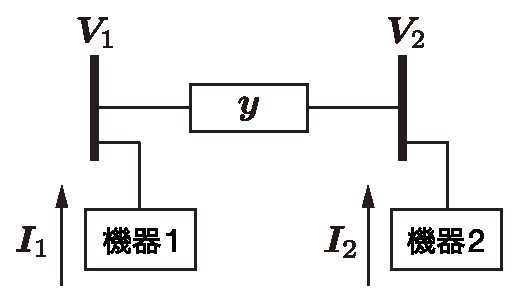
\includegraphics[width = .25\linewidth]{figs/2busex}
\medskip
\caption{2つの母線からなる電力系統\red{(図不要?)}}
\label{fig:2buspf}
\medskip
\end{figure}
\begin{例}[2つの母線で構成される電力系統モデルの潮流計算]\label{ex:2buspf}
\FIGref{fig:2buspf}の2つの母線から構成される電力系統を考えよう。
各母線には負荷または発電機が接続されているものと考えるが,以下の計算では接続される機器の種類を具体的に指定する必要はない。

2つの母線を結ぶ送電線のアドミタンスを$\bm{y}\in \mathbb{C}$とする。
基本的な送電線モデルを採用するとき,母線の電圧フェーザと電流フェーザには
\begin{align}\label{eq:exyIV}
\mat{
\bm{I}_1^{\star}\\
\bm{I}_2^{\star}
}
=
\mat{
\bm{y} & -\bm{y} \\
-\bm{y} & \bm{y}
}
\mat{
\bm{V}_1^{\star}\\
\bm{V}_2^{\star}
}
\end{align}
の関係が成り立つ。
ただし,定常状態における値であることを明示するために「${\star}$」をつけて表記した。
ここで,
式\ref{eq:defPQVIi2}の関係を用いて電流フェーザを消去すれば,式\ref{eq:exyIV}と等価な連立方程式が,定常状態における有効電力,無効電力,電圧フェーザを用いて
\begin{subequations}\label{eq:PQpf}
\begin{align}\label{eq:PQcom}
\simode{
P_1^{\star} + \bm{j} Q_1^{\star} &= 
\overline{\bm{y}} \left( 
 |\bm{V}_1^{\star}|^2 
-  |\bm{V}_1^{\star}| |\bm{V}_2^{\star}| e^{ \bm{j} (\angle \bm{V}_1^{\star}- \angle \bm{V}_2^{\star})}
\right) \\
P_2^{\star} + \bm{j} Q_2^{\star} &= 
\overline{\bm{y}} \left( 
 |\bm{V}_2^{\star}|^2
 - |\bm{V}_1^{\star}| |\bm{V}_2^{\star}| e^{ \bm{j} (\angle \bm{V}_2^{\star} - \angle \bm{V}_1^{\star})}
\right)
}
\end{align}
のように得られる。
潮流計算の目的は,この連立方程式を満たす1組の
\[
(P_1^{\star},Q_1^{\star}, |\bm{V}_1^{\star}|, \angle \bm{V}_1^{\star}, P_2^{\star},Q_2^{\star},|\bm{V}_2^{\star}|, \angle \bm{V}_2^{\star})
\]
を定めることである。

送電線のコンダクタンスとサセプタンスを
\[
g:= \real[\bm{y}],\qquad
b:= \imag[\bm{y}]
\]
と表す。
このとき,式\ref{eq:PQcom}の実部と虚部に関する方程式を考えると
\begin{align}\label{eq:PQreal}
\simode{
P_1^{\star} &= g |\bm{V}_1^{\star}|^2  
-   g |\bm{V}_1^{\star}| |\bm{V}_2^{\star}| \sfcos \angle \bm{V}_{12}^{\star}
 - b |\bm{V}_1^{\star}| |\bm{V}_2^{\star}| \sfsin \angle \bm{V}_{12}^{\star}
\\
P_2^{\star} &= g |\bm{V}_2^{\star}|^2  
-  g |\bm{V}_1^{\star}| |\bm{V}_2^{\star}| \sfcos \angle \bm{V}_{21}^{\star}
 - b |\bm{V}_1^{\star}| |\bm{V}_2^{\star}| \sfsin \angle \bm{V}_{21}^{\star}
\\
Q_1^{\star} &= - b |\bm{V}_1^{\star}|^2  
+ b |\bm{V}_1^{\star}| |\bm{V}_2^{\star}| \sfcos \angle \bm{V}_{12}^{\star} 
 - g |\bm{V}_1^{\star}| |\bm{V}_2^{\star}| \sfsin \angle \bm{V}_{12}^{\star}
\\
Q_2 &= - b |\bm{V}_2^{\star}|^2  
+ b |\bm{V}_1^{\star}| |\bm{V}_2^{\star}| \sfcos \angle \bm{V}_{21}^{\star} 
- g |\bm{V}_1^{\star}| |\bm{V}_2^{\star}| \sfsin \angle \bm{V}_{21}^{\star}
}
\end{align}
という4本の連立方程式が得られる。
\end{subequations}
ただし,$\angle \bm{V}_{ij}^{\star}:=\angle \bm{V}_i^{\star}- \angle \bm{V}_j^{\star}$である。
電圧フェーザの位相は差分値のみが意味をもつため,実質的に決定すべき変数は7個である。
したがって,式\ref{eq:PQreal}の方程式には3変数分の自由度が存在する。

これらを決定する簡単な方法は,例えば,$(|\bm{V}_1^{\star}|,|\bm{V}_2^{\star}|,\angle \bm{V}_{12}^{\star})$の3変数を適当な値に指定することである。
これにより,残りの$(P_1^{\star},P_2^{\star},Q_1^{\star},Q_2^{\star})$は式\ref{eq:PQreal}の右辺を計算するだけで決定される。
しかしながら,この方法では,各母線の電圧フェーザは任意の値に設定できる一方で,各母線に供給される電力や消費される電力を任意の値に設定することができない。
現実的な設定で数値シミュレーションを実行するためには,指定した有効電力や無効電力の値を実現するように電圧フェーザの値を適切に定めることがしばしば必要となる。

例えば,$P_1^{\star}=1$,$P_2^{\star}=-1$
を実現する$(|\bm{V}_1^{\star}|,|\bm{V}_2^{\star}|,\angle \bm{V}_{12}^{\star})$を求めることを考えてみよう。
これは,母線1に接続された機器が供給する有効電力と母線2に接続された機器が消費する有効電力が,定常状態においてどちらも1である場合に,電圧フェーザの分布を求めることに相当する。
式\ref{eq:PQreal}の$P_1^{\star}$と$P_2^{\star}$に関する方程式を足し上げれば,$P_1^{\star}+P_2^{\star}=0$であることから
\begin{align*}
\spliteq{
0 &= g \Bigl\{
 |\bm{V}_1^{\star}|^2 + |\bm{V}_2^{\star}|^2 
- 2 |\bm{V}_1^{\star}| |\bm{V}_2^{\star}| \sfcos \angle \bm{V}_{12}^{\star}
\Bigr\}\\
&=
g \Bigl\{
\left( |\bm{V}_1^{\star}| - |\bm{V}_2^{\star}| \right)^2 
+ 2 |\bm{V}_1^{\star}| |\bm{V}_2^{\star}| \bigl( 1-\sfcos \angle \bm{V}_{12}^{\star} \bigr)
\Bigr\}
}
\end{align*}
を得る。
ここで,現実的な潮流状態では,母線の電圧フェーザの位相差である$ \angle \bm{V}_{12}^{\star}$は$\left[-\frac{\pi}{2},\frac{\pi}{2}\right]$の範囲内であること
に注意されたい\footnote{
発電機の偏角差や母線の電圧フェーザの位相差が$\left[-\frac{\pi}{2},\frac{\pi}{2}\right]$の範囲を超えてしまうと正弦関数の傾きが反転するため,非現実的な有効電力の送電特性となる。
}。
このことから,$\bm{y}$の実部である送電線のコンダクタンス成分が0でない場合には,この方程式を満たす電圧フェーザは,必ず
\begin{align}\label{eq:Vequal}
|\bm{V}_1^{\star}| = |\bm{V}_2^{\star}|,\qquad
\angle \bm{V}_{12}^{\star} =0
\end{align}
を満たさなければならない。
しかしながら,式\ref{eq:Vequal}は
\[
P_1^{\star}=P_2^{\star}=0
\]
を意味することから,$g$が0でない限りは,$P_1^{\star}=1$,$P_2^{\star}=-1$は実現不可能であることが結論づけられる。
これは,送電線のコンダクタンス成分により送電損失が生じるため,$P_1^{\star}=1$,$P_2^{\star}=-1$の設定では電力の需給が系統全体でバランスしないことを表している。
このように,「すべての有効電力やすべての無効電力を特定の値に指定してしまうと,式(\ref{eq:PQpf})を満たす変数が存在しない場合があること」に注意が必要である。

以下では,簡単化のため,送電線のコンダクタンス成分が0であると仮定してみよう。
また,対地静電容量は十分に小さく,サセプタンス$b$は非正であると仮定する。
このとき,
\begin{align*}
P_1^{\star} = -b  |\bm{V}_1^{\star}| |\bm{V}_2^{\star}| \sfsin \angle \bm{V}_{12}^{\star}, \qquad
P_2^{\star}  =   b |\bm{V}_1^{\star}| |\bm{V}_2^{\star}| \sfsin \angle \bm{V}_{12}^{\star}
\end{align*}
であることから,電圧フェーザの分布は$P_1^{\star} = -P_2^{\star}$を満たすものでなければならない。
例えば,$P_1^{\star}=1$,$P_2^{\star}=-1$と指定する場合には
\begin{align*}\textstyle
|\bm{V}_1^{\star}|=\sqrt{
\frac{2}{|b|}
}
,\qquad
 |\bm{V}_2^{\star}| 
=
\sqrt{
\frac{2}{|b|}
}
\end{align*}
のように電圧フェーザの絶対値を指定することにより,電圧フェーザの位相差は
\begin{align*}
\angle \bm{V}_{12}^{\star} = \frac{\pi}{6}
\end{align*}
と定められる。
既に3変数以上の値が定められているため,無効電力は
\begin{align*}
Q_1^{\star} = 2 -\sqrt{3},\qquad
Q_2^{\star} = 2 -\sqrt{3}
\end{align*}
のように自動的に値が定まる。
\end{例}


以上のように,与えられた送電網のアドミタンス行列$\bm{Y}$に対して,
\begin{align}\label{eq:PQVgenst}
\simode{
P_1^{\star} + \bm{j} Q_1^{\star} &= 
\sum_{j=1}^{N} \overline{\bm{Y}}_{1j} |\bm{V}_1^{\star}| |\bm{V}_j^{\star} | e^{\bm{j} \bigl(\angle \bm{V}_1^{\star} - \angle \bm{V}_j^{\star} \bigr)} \\ 
& \; \;  \vdots \\
P_N^{\star} + \bm{j} Q_N^{\star} &= 
\sum_{j=1}^{N} \overline{\bm{Y}}_{Nj} |\bm{V}_N^{\star}| |\bm{V}_j^{\star} | e^{\bm{j} \bigl(\angle \bm{V}_N^{\star} - \angle \bm{V}_j^{\star} \bigr)}
}
\end{align}
で与えられる定常状態における$2N$本の連立方程式を満たす,$4N$個の定数の組
\begin{align}\label{eq:pfconst}
\bigl(
P_1^{\star},Q_1^{\star},|\bm{V}_1^{\star}|,\angle \bm{V}_1^{\star},
\ldots,
P_N^{\star},Q_N^{\star},|\bm{V}_N^{\star}|,\angle \bm{V}_N^{\star},
\bigr)
\end{align}
を1つ定める手続きが潮流計算である。
ただし,電圧フェーザの位相は相対的な値のみが意味をもつため,実質的に定めるべき変数は$(4N-1)$個である。
\ref{sec:numstep}節で上述したように,潮流計算は,系統全体で需要と供給をバランスすることが可能な電力系統モデルの平衡点を求める手続きであると解釈できる。
なお,このプロセスにおいては,発電機や負荷などの各機器の特性は考慮されておらず,各母線に対する入出力の定常値だけを求めている。
したがって,\ref{sec:numstep}節におけるステップBの計算を行ったのちに,微分代数方程式系の内部状態に関する平衡点が1つ定まることに注意されたい。
ステップBの計算は,\ref{sec:paradef}節で後述する。

%例えば,\ref{sec:loadpr}節における負荷の定インピーダンスモデルは,$(P_i,Q_i)$と$|\bm{V}_i|$の間に
%\begin{align*}
%P_i + \bm{j} Q_i = -\frac{1}{\overline{\bm{z}}_{{\rm load}i}} |\bm{V}_i|^2
%\end{align*}
%という代数的な関係を与える。
%すなわち,$\bm{z}_{{\rm load}i}$が所与の定数である場合には,2本の方程式が式\ref{eq:PQVgen}に追加されることを意味している。
%負荷が定電流モデルや定電力モデルで記述されている場合も同様である。
%\red{しかしながら.... なぜそうしない?データシートで与えられているのが普通PQだから?}
%ただし,式(\ref{eq:gendynVI})の発電機の定常状態は機械的トルク$P_{{\rm mech}i}$と界磁電圧$V_{{\rm field}i}$という別の2変数にも依存するため,発電機の動特性に由来する方程式を潮流計算で考慮する必要はない。
%このことは\ref{sec:stagen}節で後述する。




\subsection{潮流状態の数値的な探索手法}


一般に,\red{電気学会標準モデル,IEEE 39母線系統モデル\cite{athay1979practical},IEEE 68母線系統モデル\cite{singh2013ieee}}などには,各送電線のインピーダンス値に加えて,各発電機母線に供給される電力や各負荷母線で消費される電力の標準的な値がデータシートとして与えられている。
それらの標準的な値に基づき$2N$個の変数を指定することによって,残りの変数を数値的に求めることができる。


データシートには,各負荷母線で消費される有効電力と無効電力の値,および,各発電機母線に供給される有効電力の値とその母線における電圧フェーザの絶対値が与えられているのが一般的である。
したがって,それらの値を用いることにより,$2N$個の定常値をあらかじめ指定することができる。
しかしながら,例\ref{ex:2buspf}で示されているように,すべての母線における有効電力の定常値を事前に指定してしまうと,送電損失の影響によって,残りの変数をいかなる値にしても式\ref{eq:PQVgen}の連立方程式が満たされない場合がある。
例えば,一部の負荷母線における有効電力や無効電力の値をデータシートとは異なる定常値に指定すると,発電機母線に供給されるべき有効電力や無効電力の定常値も変わると同時に,送電網を流れる電力や母線電圧フェーザの定常値も変化するため,系統全体での送電損失の合計値も変化する。
したがって,すべての発電機母線における有効電力の定常値を事前に指定してしまうと,式\ref{eq:PQVgen}の連立方程式が一般に可解とならない。


この問題を解決するための代表的な方策は,\emph{スラック母線}(slack bus)と呼ばれる特別な発電機母線を1つ導入することである。
スラック母線では,有効電力を指定する代わりに,電圧フェーザの位相を指定する。
このとき,各母線における電圧フェーザの位相は相対的な値のみが意味をもつため,スラック母線の位相の定常値を0に指定しても一般性を失わない。
結果として,系統全体での送電損失の値に整合するように,スラック母線における有効電力が自動的に決定される。
以上の手順は,つぎのようにまとめられる。
\begin{itemize}
\item[(a)] データシートに基づき,スラック母線には$(|\bm{V}_{i_0}^{\star}|,\angle \bm{V}_{i_0}^{\star})$の値,それ以外の発電機母線には$(P_i^{\star},|\bm{V}_{i}^{\star}|)_{i \in \mathcal{I}_{\rm G}\setminus\{i_0\} }$の値,負荷母線には$(P_i^{\star},Q_i^{\star})_{i \in \mathcal{I}_{\rm L}}$の値を指定する。
\item[(b)] 式\ref{eq:PQVgen}の連立方程式を満たすように,その他の変数を数値的に探索する。
\end{itemize}
ただし,$\mathcal{I}_{\rm G}$は発電機母線の添字集合,$\mathcal{I}_{\rm L}$は負荷母線の添字集合,$i_0 \in \mathcal{I}_{\rm G}$はスラック母線の添字を表す。


\begin{例}[データシートに基づく潮流計算]
\red{2つの母線の例で送電ロスがある場合?}
\end{例}



\begin{例}[経済性を考慮した潮流計算]\label{ex:pflow}
\red{発電機2つ,負荷1つとかで,スラック母線を変えると決定される発電量が送電ロスなどで変わることを見せる?}
\end{例}


\subsection{潮流計算の実装法}

MATLABを用いて潮流計算を行うプログラムを実装する方法について説明する。
潮流計算のためには,式\ref{eq:ohmY2}の連立方程式を解く必要がある。
そこで,まずは電力システムではない簡単な例題を用いて,連立方程式をMATLABで解く方法を示す。
\subsubsection{簡単な例題}
代数方程式
\begin{subequations}\label{eq:algeblaic_equation_ex1}
\begin{align}
x^2 - y = 0\\
x^2 + y^2 - 2 = 0
\end{align}
\end{subequations}
を満たす$(x, y)$の組を数値計算によって求めることを考えよう。
ここで,この解は$(x, y) = (-1, 1), (1, 1)$の2つであることに注意しよう。
MATLABで代数方程式を解くためには,\texttt{optimization toolbox}の\texttt{fsolve}
コマンドが便利である。このコマンドを用いるためには,代数方程式$f(x)=0$の$f(x)$にあたる部分,
すなわち,式\eqref{eq:algebraic_eqation_ex1}の左辺を評価する関数を実装する必要がある。
この関数を\texttt{funce\_x1.m}という名前のファイルとして実装すると,
プログラム\nobreak\ref{program:ex1}のようになる。

\begin{PROGRAMA}[count,title={func\_ex1.m}]\label{program:ex1}
\begin{verbatim}
function out = func_ex1(x_in)

x = x_in(1);
y = x_in(2);

out = zeros(2, 1);
out(1) = x^2 - y;
out(2) = x^2 + y^2 - 2;

end
\end{verbatim}
\end{PROGRAMA}

つぎに,この関数を用いて\texttt{fsolve}を実行し,代数方程式を解くプログラムを記述すると,
プログラム\nobreak\ref{program:ex1_main}となる。
\begin{PROGRAMA}[count,title={main\_ex1.m}]\label{program:ex1_main}
\begin{verbatim}
options = optimoptions('fsolve', 'Display', 'iter');
x0 = [0.1; 0.5];
x_sol = fsolve(@func_ex1, x0, options)
\end{verbatim}
\end{PROGRAMA}

ここで,\texttt{options}は最適化を行うときのオプションを設定しており,
この例では最適化の過程を画面に表示することを示している。また,
プログラムにおいて\texttt{x0 = [0.1; 0.5];}は
数値計算によって最適化を行う際の初期値を表している。
このプログラムを実行すると,つぎの実行結果が得られる。

\begin{実行結果}
\begin{verbatim}
                        Norm of      First-order   Trust-region
  Iteration  Func-count     f(x)          step         optimality    radius
      0          3          3.2677                          1.25               1
      1          6        0.282554              1          0.757               1
\end{verbatim}
\omitcode
\begin{verbatim}
  4         15     3.60447e-14    0.000367541       5.37e-07             2.5

  方程式が解かれました。
\end{verbatim}
\omitcode
\begin{verbatim}
  x_sol =
      1.0000
      1.0000
\end{verbatim}
\end{実行結果}


この結果から,解のうちの一つである$(x, y) = (1, 1)$が得られていることがわかる。
\texttt{fsolve}を用いた数値解法では,すべての
解を得られるわけではなく,解のうちのどれか
一つが得られるに過ぎないことに注意しよう。
ここで,この初期値として
\texttt{x0 = [-0.1; 0.5];}
を設定した場合の結果をつぎに示す。

\begin{実行結果}
\begin{verbatim}
  方程式が解かれました。

  関数値のベクトルがゼロに近く 
  (関数の許容誤差値による測定)、
  問題が正則として現れる (勾配による測定) ため、fsolve は完了しました。
  
  <停止条件の詳細>
  x_sol =
     -1.0000
      1.0000
\end{verbatim}
\end{実行結果}

この結果では,もう一つの解$(x, y) = (-1, 1)$が得られていることがわかる。
このように,数値解法を用いる非凸な最適化では,初期値によって異なる解が得られることに注意が必要である。
さらに別の例として,\texttt{x0 = [-0.1; -0.1];}
とした場合の実行結果を見てみよう。



% \begin{例}[MATLABによる実装例]
%   \newcommand{\thshift}{\theta}
%   % 例\ref{ex:transformer_typeY}で導出したアドミタンス行列において,
%   % $\tau = 1$, $\thshift=0$とおけば,例\ref{ex:pitypeY}の結果が得られる。
%   % また,さらに$b=0$とおけば,例\ref{ex:derY}の結果となる。
%   % このことから,これまでのモデルでは例\ref{ex:transformer_typeY}が
%   % 最も一般的なモデルであるといえる。
%   ここでは,例\ref{ex:transformer_typeY}におけるアドミタンス行列の
%   作成をMATLABで実装する例を示す。


% \end{例}

\subsection{アドミタンス行列と送電損失の関係\advanced}

以下では,$N$個の母線で構成される一般的な送電網に対して,潮流状態に関する送電損失の数学的表現を導出する。
対称なコンダクタンス行列とサセプタンス行列をもつアドミタンス行列$\bm{Y}$は,適当な定数$\phi_{ij}=\phi_{ji}$,$\psi_{ij}=\psi_{ji}$を用いて,
\begin{align}
\spliteq{
\real \left[\bm{Y} \right]
& =
\mat{
  \sum_{j=1}^{N} \phi_{1j} & -\phi_{12} & \cdots & -\phi_{1N}\\
  -\phi_{21} & \sum_{j=1}^{N} \phi_{2j} & \cdots & -\phi_{2N}\\
  \vdots & \vdots & \ddots & \vdots\\
  -\phi_{N1} & -\phi_{N2} & \cdots & \sum_{j=1}^{N} \phi_{Nj}
},
\\
\imag \left[\bm{Y} \right]
& =
-\mat{
  \sum_{j=1}^{N} \psi_{1j} & -\psi_{12} & \cdots & -\psi_{1N}\\
  -\psi_{21} & \sum_{j=1}^{N} \psi_{2j} & \cdots & -\psi_{2N}\\
  \vdots & \vdots & \ddots & \vdots\\
  -\psi_{N1} & -\psi_{N2} & \cdots & \sum_{j=1}^{N} \psi_{Nj}
}
}
\end{align}
の形式で書き表すことができる。
この形式は,コンダクタンス行列とサセプタンス行列の第$(i,j)$要素をそれぞれ$G_{ij}$,$B_{ij}$と表したとき
\[
\phi_{ij}:=-G_{ij},\qquad 
\phi_{ii}:= \sum_{j=1}^N G_{ij},\qquad
\psi_{ij}:=B_{ij},\qquad 
\psi_{ii}:= - \sum_{j=1}^N B_{ij}
\]
と定義していることに等しい。
この表現を用いるとつぎの事実が示される。

\begin{定理}[送電損失の母線電圧フェーザによる表現]
\label{thm:PQ}
式\ref{eq:PQVgen}に対して,系統全体での有効電力と無効電力の送電損失として
\begin{align}
L_{P}(t) := P_1(t) +\cdots P_N(t)
,\qquad
L_Q(t) := Q_1(t) +\cdots Q_N(t)
\end{align}
を定義する。
これらの送電損失は
\begin{align}
\spliteq{
L_P(t) &= \sum_{i=1}^N \phi_{ii} |\bm{V}_{i}(t)|^2  +
\sum_{i=1}^N \sum_{j=1}^N
\phi_{ij} 
W\bigl(\bm{V}_i(t),\bm{V}_j(t)\bigr)
\\
L_Q(t) &= \sum_{i=1}^N \psi_{ii} |\bm{V}_{i}(t)|^2  +
\sum_{i=1}^N \sum_{j=1}^N
\psi_{ij} 
W\bigl(\bm{V}_i(t),\bm{V}_j(t)\bigr)
}
\end{align}
で与えられる。
ただし,
\[
W(\bm{V}_i,\bm{V}_j):=
\frac{1}{2} \left( |\bm{V}_i| - |\bm{V}_j| \right)^2 
+  |\bm{V}_i| |\bm{V}_j| \bigl\{ 1-\sfcos (\angle \bm{V}_i- \angle \bm{V}_j) \bigr\}
\]
とする。
\end{定理}


定理\ref{thm:PQ}は,例\ref{ex:2buspf}で示されている2母線の電力系統における電力損失の議論が,任意の個数の母線から構成される電力系統にも同様に一般化できることを示している。
ここで,\ref{sec:admathp}節のようにアドミタンス行列$\bm{Y}$を
\[
\bm{Y}=\bm{Y}_0 + \bm{j} \sfdiag(\beta_i)_{i\in \{1,\ldots,N\} }
\]
と表す場合には,$\bm{Y}_0 \mathds{1}=0$であることから,
$\phi_{ii}=0$,
$\psi_{ii}= - \beta_i$
となる。
また,各送電線のコンダクタンスは非負であり,サセプタンスは負であることから,すべての$i\neq j$に対して,$\phi_{ij} $と$\psi_{ij}$は非負である。
したがって,$\phi_{ij}$が0でない限りは,母線$i$と母線$j$の間で有効電力を送電する場合に必ず電力損失が生じることがわかる。
これにより,系統全体での有効電力の送電損失$L_P(t)$は,任意の時刻$t$で正であることがわかる。
\red{同様に,$\beta_i$が十分に小さい場合,すなわち,送電線の対地静電容量が十分に小さい場合には,無効電力の送電損失$L_Q(t)$も正であることがわかる。
}
\blue{コンデンサの挿入により無効電力を供給することに対応?}

\section{所与の潮流状態を実現する各機器のパラメータ設定}\label{sec:paradef}

本節では,\ref{sec:numstep}節のステップBとして説明された,潮流計算の結果に整合するように発電機の内部状態の定常値や外部入力値,負荷のパラメータ値を逆算する方法を説明する。


\subsection{所望の電力供給を実現する発電機の定常状態}\label{sec:stagen}

\ref{sec:genfund}節における電圧フェーザを入力とする発電機モデルを考えよう。
表記の簡単化のため,添字$i$を省略して
\begin{align}\label{eq:gendif_}
\simode{
\dot{\delta}&= \omega_0  \Delta \omega\\
M   \Delta \dot{\omega}&= 
 - D \Delta\omega  
 - P
+P_{{\rm mech}}
\\
\tau_{{\rm d}} \dot{E} & = 
 -\tfrac{X_{{\rm d}}}{X_{{\rm q}}}E
+\left(
\tfrac{X_{{\rm d}}}{X_{{\rm q}}}-1
\right)
|\bm{V}| \sfcos (\delta - \angle \bm{V} ) 
+ V_{{\rm field}}
}
\end{align}
とする。
ここで,有効電力と無効電力を出力とする場合には
\begin{align}\label{eq:PQout_}
\spliteq{
P &=  \frac{|\bm{V} | E}{X_{{\rm q}}} \sfsin(\delta -  \angle \bm{V}), \\
Q &=  \frac{|\bm{V}|E}{X_{{\rm q}}} \sfcos (\delta - \angle \bm{V})
-\frac{|\bm{V}|^2}{X_{{\rm q}} }
}
\end{align}
である。
%また,電流フェーザを出力とする場合には
%\begin{align}\label{eq:phVIsincosC2_}
%\spliteq{
% |\bm{I}| \sfcos (\delta -\angle \bm{I}) & =
%\frac{|\bm{V}|}{X_{{\rm q}}}  \sfsin (\delta -\angle \bm{V}) , \\
%|\bm{I}| \sfsin (\delta -\angle \bm{I})
%& = \frac{E - |\bm{V}| \sfcos (\delta -\angle \bm{V}) }{X_{{\rm q}}} 
%}
%\end{align}
%である。
ここでの目的は,潮流計算の結果として,発電機が接続される母線の有効電力,無効電力,電圧フェーザの絶対値と位相が定数で与えられた場合に,それらの値に整合する発電機の内部状態と外部入力値の定常値を求めることである。
具体的には,与えられた有効電力,無効電力,電圧フェーザの絶対値と位相の組を$(P^{\star},Q^{\star},|V^{\star}|,\angle \bm{V}^{\star})$と表すとき,
\begin{align}\label{eq:P0Q0eq}
\simode{
P^{\star} &=  \tfrac{|V^{\star}| E^{\star}}{X_{{\rm q}}} \sfsin(\delta^{\star} -  \angle \bm{V}^{\star}), \\
Q^{\star} & = \tfrac{|V^{\star}| E^{\star}}{X_{{\rm q}}} \sfcos (\delta^{\star} -  \angle \bm{V}^{\star})
-\tfrac{|V^{\star}|^2}{X_{{\rm q}} }, \\
0 & =  - P^{\star} +P_{{\rm mech}}^{\star}, \\
0 & = 
 -\tfrac{X_{{\rm d}}}{X_{{\rm q}}}E^{\star}
+\left(
\tfrac{X_{{\rm d}}}{X_{{\rm q}}}-1
\right)
|V^{\star}| \sfcos (\delta^{\star} - \angle \bm{V}^{\star})
+ V_{{\rm field}}^{\star}
}
\end{align}
の連立方程式を満たす発電機の内部状態の定常値$(\delta^{\star},E^{\star})$と外部入力の定常値$(P_{{\rm mech}}^{\star},V_{{\rm field}}^{\star})$を求める。
式\ref{eq:P0Q0eq}の連立方程式は,式\ref{eq:gendif_}において周波数偏差$\Delta \omega$の定常値が0であるとした場合の平衡点に関する方程式である。
また,与えられた$(P^{\star},Q^{\star},|V^{\star}|,\angle \bm{V}^{\star})$は,各母線に対する発電機モデルの入出力値に対応している。


式\ref{eq:P0Q0eq}を満たす発電機の内部状態の定常値を具体的に計算すると
\begin{subequations}\label{eq:intssgen}
\begin{align}
\spliteq{
\delta ^{\star} &= \angle \bm{V}^{\star}
+ \sfarctan \left( \frac{P^{\star}}{Q^{\star} + \frac{ |\bm{V}^{\star}|^2}{X_{\rm q}} } \right), 
\\
E^{\star} &= 
\frac{X_{\rm q}}{ |\bm{V}^{\star}| } \sqrt{ \left( Q^{\star} + \frac{|\bm{V}^{\star}|^2}{X_{\rm q}} \right)^2 + (P^{\star})^2 } 
}
\end{align}
となる。
また,機械的トルクと界磁電圧の定常値は
\begin{align}\label{eq:PmVfdss}
\spliteq{
P_{{\rm mech}}^{\star} &=    P^{\star}, \\
 V_{{\rm field}}^{\star} &=  \frac{ \frac{X_{\rm d}}{ |\bm{V}^{\star}| } \left\{ \left( Q^{\star} + \frac{|\bm{V}^{\star}|^2}{X_{\rm q}} \right) 
\left(Q^{\star} + \frac{|\bm{V}^{\star}|^2}{X_{\rm d}} \right) +(P^{\star})^2  \right\} }
{  \sqrt{ \left( Q^{\star} + \frac{|\bm{V}^{\star}|^2}{X_{\rm q}} \right)^2 + (P^{\star})^2 }  }
}
\end{align}
となる。
\end{subequations}
これらの導出過程は,\ref{sec:genssPQ}節を参照されたい。

\subsection{所望の電力消費を実現する負荷のパラメータ}\label{sec:loadpara}

式\ref{eq:defPQVIi2}を用いて電流フェーザを消去すると,定インピーダンスモデルは,
\begin{subequations}\label{eq:lmodels}
\begin{align}
P + \bm{j} Q = -\frac{1}{\overline{\bm{z}}_{\rm load}^{\star}} |\bm{V}|^2
\end{align}
と書き表される。
ただし,母線の添字$i$は表記の簡単化のため省略した。
これは電流フェーザ$\bm{V}$を入力,有効電力$P$と無効電力$Q$を出力とした場合の負荷の定インピーダンスモデルと解釈できる。
潮流計算により定められた有効電力と無効電力の値を$P^{\star}$と$Q^{\star}$,電圧フェーザの絶対値を$|\bm{V}^{\star}|$と表せば,負荷のインピーダンス$\bm{z}_{\rm load}^{\star}$の実部と虚部はそれぞれ
\begin{align*}
\real [\bm{z}_{\rm load}^{\star}] = - \frac{ P^{\star}}{(P^{\star})^2 + (Q^{\star})^2}|\bm{V}^{\star}|^2
,\quad
\imag [\bm{z}_{\rm load}^{\star}] = - \frac{ Q^{\star}}{(P^{\star})^2 + (Q^{\star})^2}|\bm{V}^{\star}|^2
\end{align*}
と求められる。
同様に,定電流モデルは
\begin{align}
P + \bm{j} Q = \overline{\bm{I}}_{\rm load}^{\star} \bm{V}
\end{align}
と書き表されることから,負荷の電流パラメータの実部と虚部はそれぞれ
\begin{align*}
\red{
\real [\bm{I}_{\rm load}^{\star}]
 =\frac{P^{\star} }{|\bm{V}^{\star}|},\qquad
\imag [\bm{I}_{\rm load}^{\star}]
 = -\frac{ Q^{\star} }{|\bm{V}^{\star}|}
 }
\end{align*}
と求められる。
ただし,$\angle \bm{V}^{\star}$は潮流計算で定められた母線の電圧フェーザの位相である。
定電力モデルは
\begin{align}
P + \bm{j} Q =
P_{{\rm load}}^{\star} + \bm{j} Q_{{\rm load}}^{\star} 
\end{align}
\end{subequations}
であることから,明らかにそのパラメータは
\begin{align*}
P_{\rm load}^{\star}=P^{\star}
,\qquad
Q_{\rm load}^{\star}=Q^{\star}
\end{align*}
である。
式(\ref{eq:lmodels})のパラメータ値を負荷モデルに設定すれば,潮流計算によって求められた潮流状態が定常的に実現される。

\subsection{発電機の内部状態と入出力の数学的関係\advanced}\label{sec:genssPQ}

以下では,発電機の内部状態,母線に供給される有効電力と無効電力,母線の電圧フェーザの間に成り立つ関係を数学的に解析する。
ここでは,\ref{sec:genmodadv}節で扱った\red{突極型}の発電機モデルを用いる。
ただし,表記の簡単化のため,添字$i$を省略して
\begin{align}\label{eq:gendif}
\simode{
\dot{\delta}&= \omega_0  \Delta \omega\\
M   \Delta \dot{\omega}&= 
 - D \Delta\omega  
 - P
+P_{{\rm mech}}
\\
\tau_{{\rm d}} \dot{E} & = 
 -\tfrac{X_{{\rm d}}}{X_{{\rm d}}'}E
+\left(
\tfrac{X_{{\rm d}}}{X_{{\rm d}}'}-1
\right)
|\bm{V}| \sfcos (\delta - \angle \bm{V} ) 
+ V_{{\rm field}}
}
\end{align}
とする。
ここで,有効電力と無効電力を出力とする場合には
\begin{align}\label{eq:PQout}
\spliteq{
P &=  \frac{|\bm{V} | E}{X_{{\rm d}}'} \sfsin(\delta -  \angle \bm{V})
-  
\left( \frac{1}{X_{{\rm d}}'}  -  \frac{1}{X_{{\rm q}}} \right)
|\bm{V}|^2 \sfsin( \delta - \angle \bm{V})\sfcos( \delta - \angle \bm{V}), \\
Q &=  \frac{|\bm{V}|E}{X_{{\rm d}}'} \sfcos (\delta - \angle \bm{V})
-|\bm{V}|^2 \left( \frac{\sfcos^2 (\delta - \angle \bm{V}) }{X_{{\rm d}}'} 
+ \frac{\sfsin^2 (\delta - \angle \bm{V})}{X_{{\rm q}}} \right)
}
\end{align}
である。
明らかに,過渡リアクタンスを$X_{{\rm d}}'=X_{{\rm q}}$とすれば,\ref{sec:stagen}節で扱った発電機モデルに一致する。
また,電流フェーザを出力とする場合には
\begin{align}\label{eq:phVIsincosC2}
\spliteq{
 |\bm{I}| \sfcos (\delta -\angle \bm{I}) & =
\frac{|\bm{V}|}{X_{{\rm q}}}  \sfsin (\delta -\angle \bm{V}) , \\
|\bm{I}| \sfsin (\delta -\angle \bm{I})
& = \frac{E - |\bm{V}| \sfcos (\delta -\angle \bm{V}) }{X_{{\rm d}}'} 
}
\end{align}
である。
なお,式\ref{eq:PQout}と式\ref{eq:phVIsincosC2}は等価な出力であること,すなわち,与えられた任意の$(\delta, E, |\bm{V}|, \angle \bm{V})$に対して,$(P,Q)$と$(|\bm{I}|, \angle \bm{I})$には一対一の関係が存在することに注意されたい。

この発電機モデルに対して,つぎの事実が示される。

\begin{補題}[発電機の内部状態と入出力の関係]\label{lem:delVE}
式\ref{eq:PQout}を$\delta - \angle \bm{V}$と$E$に関する連立方程式と考えるとき,その解は
\begin{align}\label{eq:tandelV}
\spliteq{
\delta - \angle \bm{V} & = \sfarctan  \left( \frac{P}{Q + \frac{ |\bm{V}|^2}{X_{\rm q}} } \right) , \\
E &=
\frac{ \frac{X_{\rm d}'}{|\bm{V}| } \left\{ \left( Q + \frac{|\bm{V}|^2}{X_{\rm q}} \right) \left(Q + \frac{|\bm{V}|^2}{X_{\rm d}'} \right) +P^2  \right\} }
{  \sqrt{ \left( Q + \frac{|\bm{V}|^2}{X_{\rm q}} \right)^2 + P^2 }  }
}
\end{align}
%\begin{align}\label{eq:tandelV}
%\spliteq{
%\delta(t) - \angle \bm{V}(t) & = \sfarctan  \left( \frac{P(t)}{Q(t) + \frac{ |\bm{V}(t)|^2}{X_{\rm q}} } \right) , \\
%E(t) &=
%\frac{ \frac{X_{\rm d}'}{|\bm{V}(t)| } \left\{ \left( Q(t) + \frac{|\bm{V}(t)|^2}{X_{\rm q}} \right) \left(Q(t) + \frac{|\bm{V}(t)|^2}{X_{\rm d}'} \right) +P^2(t)  \right\} }
%{  \sqrt{ \left( Q(t) + \frac{|\bm{V}(t)|^2}{X_{\rm q}} \right)^2 + P^2(t) }  }
%}
%\end{align}
で与えられる。
ただし,$|\bm{V}|\neq 0$とする。
逆に,式\ref{eq:tandelV}を$P$と$Q$に関する連立方程式と考えるとき,その解は式\ref{eq:PQout}で与えられる。
\end{補題}

\begin{証明}
まず,式\ref{eq:PQout}から式\ref{eq:tandelV}を導く。
式\ref{eq:PQout}の$P$に$\sfcos (\delta - \angle \bm{V})$を乗じ,
$Q$に$\sfsin (\delta - \angle \bm{V})$を乗じて差をとれば
\begin{align*}
P \sfcos (\delta - \angle \bm{V}) - Q \sfsin (\delta - \angle \bm{V})
= \frac{|\bm{V}|^2}{X_{\rm q}} \sfsin (\delta - \angle \bm{V}) 
\end{align*}
が得られる。
これにより,式\ref{eq:tandelV}左の関係が得られる。
つぎに,式\ref{eq:tandelV}右の関係を示す。
式\ref{eq:defPQVIi2}を用いて$P$と$Q$を$\bm{I}$で書き直すと,式\ref{eq:PQout}は式\ref{eq:phVIsincosC2}に等価変形される。
また,これは
\begin{align}\label{eq:tmpVE}
|\bm{V}|e^{\bm{j}(\delta - \angle \bm{V})}=E
-X_{\rm d}' |\bm{I}| \sfsin (\delta - \angle \bm{I})
+ 
\bm{j} X_{\rm q} 
|\bm{I}| \sfcos (\delta - \angle \bm{I})
\end{align}
と等価である。
式\ref{eq:tandelV}左の関係を複素数で表現すると
\begin{align*}
\frac{ e^{\bm{j}(\delta - \angle \bm{V})} - e^{-\bm{j}(\delta - \angle \bm{V})}}
{e^{\bm{j}(\delta - \angle \bm{V})} + e^{-\bm{j}(\delta - \angle \bm{V})}}
= 
\underbrace{
\frac{P}{Q + \frac{ |\bm{V}|^2}{X_{\rm q}} }
}_{\alpha}
 \bm{j}
\end{align*}
であることから
\begin{align*}
e^{-\bm{j}(\delta - \angle \bm{V})} = \frac{1-\alpha \bm{j}}{1+\alpha \bm{j}}
e^{\bm{j}(\delta - \angle \bm{V})}
\end{align*}
がわかる。
したがって,式\ref{eq:defPQVIi2}を等価変形した
\begin{align}\label{eq:IVPQ}
|\bm{I}|e^{\bm{j}(\delta - \angle \bm{I})} = \frac{P+\bm{j}Q}{|\bm{V}|}  
e^{\bm{j}(\delta - \angle \bm{V})}
\end{align}
について,その複素共役を考えることにより
\begin{align}\label{eq:IVPQc}
|\bm{I}|e^{-\bm{j}(\delta - \angle \bm{I})} = \frac{P-\bm{j}Q}{|\bm{V}|}  
\cdot \frac{1-\alpha \bm{j}}{1+\alpha \bm{j}}
e^{\bm{j}(\delta - \angle \bm{V})}
\end{align}
を得る。
式\ref{eq:IVPQ}と式\ref{eq:IVPQc}から
\begin{align*}
|\bm{I}| \sfsin (\delta - \angle \bm{I})
& =
\frac{1}{|\bm{V}|} \cdot
\frac{\alpha P +Q}{ 1+\alpha \bm{j} }e^{\bm{j}(\delta - \angle \bm{V})}, \\
|\bm{I}| \sfcos (\delta - \angle \bm{I})
& =
\frac{1}{|\bm{V}|} \cdot
\frac{ P - \alpha Q}{ 1+\alpha \bm{j} }e^{\bm{j}(\delta - \angle \bm{V})}
\end{align*}
がわかる。
これらを式\ref{eq:tmpVE}に代入することによって,$\bm{I}$を$P$と$Q$で改めて書き直せば,式\ref{eq:tandelV}左の関係が成り立つとき,式\ref{eq:PQout}が
\begin{align}\label{eq:Etran}
E=
\frac{X_{\rm d}'}{|\bm{V}| } 
\left\{
\left(Q + \frac{|\bm{V}|^2}{X_{\rm q}} \right) \left(Q + \frac{|\bm{V}|^2}{X_{\rm d}'} \right) +P^2
\right\}
\frac{  Q + \frac{|\bm{V}|^2}{X_{\rm q}} - \bm{j} P }
{   \left( Q + \frac{|\bm{V}|^2}{X_{\rm q}} \right)^2 + P^2   }
e^{\bm{j}(\delta - \angle \bm{V})}
\end{align}
と等価であることがわかる。
ここで,式\ref{eq:tandelV}左の関係から
\begin{align*}
Q + \frac{|\bm{V}|^2}{X_{\rm q}} - \bm{j} P
= 
\left|Q + \frac{|\bm{V}|^2}{X_{\rm q}} - \bm{j} P \right|
e^{-\bm{j}(\delta - \angle \bm{V})}
\end{align*}
がわかる。
以上より,式\ref{eq:tandelV}右の関係が得られる。

逆の手順をたどって,式\ref{eq:tandelV}から式\ref{eq:PQout}を導く。
式\ref{eq:tandelV}左の関係を用いると,式\ref{eq:tandelV}右の$E$は式\ref{eq:Etran}の$E$で書き換えられる。
前述のように,式\ref{eq:tandelV}左の関係が成り立つとき,式\ref{eq:Etran}は式\ref{eq:PQout}と等価である。
\end{証明}

補題\ref{lem:delVE}は,変数の組$(\delta - \angle \bm{V},E)$と組$(P,Q)$の間に一対一の関係があることを示している。
特に,発電機の入出力である$(|\bm{V}|,\angle \bm{V})$や$(P,Q)$から,発電機の内部状態である$(\delta,E)$を一意的に逆算できることを示している。
なお,式\ref{eq:tandelV}の関係は定常状態,過渡状態に関わらず任意の時刻$t$で成り立つことに注意されたい。

つぎの定理は,発電機の定常状態において,入力,出力,および,内部状態の間に成り立つ関係を与える。

\begin{定理}[定常状態における発電機の内部状態と入出力の関係]
\label{thm:stst}
式\ref{eq:gendif}および式\ref{eq:PQout}の発電機モデルを考える。
ある実定数$|\bm{V}^{\star}|$,$\Delta \omega^{\star}$,$\angle \bm{V}^{\star}$,$P^{\star}$,$Q^{\star}$に対して,機械的トルクと界磁電圧による入力を
\begin{subequations}\label{eq:allinputs}
\begin{align}\label{eq:PmVfd}
\spliteq{
P_{{\rm mech}}(t) &=   D \Delta \omega^{\star}  + P^{\star}, \\
 V_{{\rm field}}(t) &=  \frac{ \frac{X_{\rm d}}{ |\bm{V}^{\star}| } \left\{ \left( Q^{\star} + \frac{|\bm{V}^{\star}|^2}{X_{\rm q}} \right) 
\left(Q^{\star} + \frac{|\bm{V}^{\star}|^2}{X_{\rm d}} \right) +(P^{\star})^2  \right\} }
{  \sqrt{ \left( Q^{\star} + \frac{|\bm{V}^{\star}|^2}{X_{\rm q}} \right)^2 + (P^{\star})^2 }  }
}
\end{align}
で与えられる定数とし,母線の電圧フェーザによる入力が
\begin{align}\label{eq:busvolin}
|\bm{V}(t)|=|\bm{V}^{\star}|,\qquad
\angle \bm{V}(t) = \omega_0 \Delta \omega^{\star} t + \angle \bm{V}^{\star}
\end{align}
\end{subequations}
と定められているものとする。
このとき,回転子偏角,周波数偏差,内部電圧は
\begin{align}\label{eq:inicon}
\spliteq{
\delta (t) &= \angle \bm{V}(t)
+ \sfarctan \left( \frac{P^{\star}}{Q^{\star} + \frac{ |\bm{V}^{\star}|^2}{X_{\rm q}} } \right), 
\\
\Delta \omega(t) &= \Delta \omega^{\star},
\\
E(t) &= \frac{ \frac{X_{\rm d}'}{ |\bm{V}^{\star}| } \left\{ \left( Q^{\star} + \frac{|\bm{V}^{\star}|^2}{X_{\rm q}} \right) 
\left(Q^{\star} + \frac{|\bm{V}^{\star}|^2}{X_{\rm d}' } \right) +(P^{\star})^2  \right\} }
{  \sqrt{ \left( Q^{\star} + \frac{|\bm{V}^{\star}|^2}{X_{\rm q}} \right)^2 + (P^{\star})^2 }  }
}
\end{align}
を定常解にもつ。
また,母線に供給される有効電力と無効電力は
\begin{align}\label{eq:PtQt}
P(t)=P^{\star},\qquad
Q(t)=Q^{\star}
\end{align}
で与えられる定数となる。
\end{定理}

\begin{証明}
まず,式(\ref{eq:allinputs})の入力のもとで,式\ref{eq:inicon}が式\ref{eq:gendif}の微分方程式の解であることを仮定した場合に,出力に関して式\ref{eq:PtQt}が成り立つことを示す。
補題\ref{lem:delVE}で示されているように,式\ref{eq:inicon}を$P^{\star}$と$Q^{\star}$に関する方程式と考えれば,それらの解は
\begin{align*}
\spliteq{
P^{\star} &=  \frac{|\bm{V}^{\star}| E(t)}{X_{{\rm d}}'} \sfsin\left(\delta(t) -  \angle \bm{V}(t)\right) 
\\
& -  
\left( \frac{1}{X_{{\rm d}}'}  -  \frac{1}{X_{{\rm q}}} \right)
|\bm{V}^{\star}|^2 \sfsin\left( \delta(t) - \angle \bm{V}(t) \right) \sfcos\left( \delta(t) - \angle \bm{V}(t) \right), 
\\
Q^{\star} &=  \frac{|\bm{V}^{\star}| E(t)}{X_{{\rm d}}'} \sfcos \left( \delta(t) - \angle \bm{V}(t) \right)
\\
& - |\bm{V}^{\star}|^2 \left( \frac{\sfcos^2 \left( \delta(t) - \angle \bm{V}(t) \right) }{X_{{\rm d}}'} 
+ \frac{\sfsin^2 \left( \delta(t) - \angle \bm{V}(t) \right)}{X_{{\rm q}}} \right)
}
\end{align*}
で与えられる。
これは式\ref{eq:PtQt}を意味している。

つぎに,式(\ref{eq:allinputs})の入力のもとで,式\ref{eq:inicon}が式\ref{eq:gendif}の微分方程式の解であることを確かめる。
式\ref{eq:gendif}の$\delta$と$\Delta \omega$に関する微分方程式は
\begin{align*}
\frac{M}{\omega_0} \ddot{\delta}(t) + \frac{D}{\omega_0} \dot{\delta}(t)
+ P(t) - P_{{\rm mech}}(t) = 0
\end{align*}
と等価である。
式\ref{eq:PmVfd}の$P_{{\rm mech}}(t)$,式\ref{eq:PtQt}の$P(t)$,式\ref{eq:inicon}の$\delta(t)$を代入すれば,それらがこの微分方程式を満たすことが確かめられる。
同様に,式\ref{eq:PmVfd}の$V_{{\rm field}}(t)$,式\ref{eq:inicon}の$\delta(t) - \angle \bm{V}(t)$と$E(t)$を代入することにより,式\ref{eq:gendif}の$E$に関する微分方程式が満たされることがわかる。
ただし
\begin{align*}
\sfcos \left( \sfarctan \left( \frac{P^{\star}}{Q^{\star} + \frac{ |\bm{V}^{\star}|^2}{X_{\rm q}} } \right) \right) =
\frac{ Q^{\star} + \frac{|\bm{V}^{\star}|^2}{X_{\rm q}} }
{  \sqrt{ \left( Q^{\star} + \frac{|\bm{V}^{\star}|^2}{X_{\rm q}} \right)^2 + (P^{\star})^2 }  }
\end{align*}
である。
以上より,求める結果がしたがう。
\end{証明}

定理\ref{thm:stst}から,潮流計算によって定められた母線の電圧フェーザ,有効電力,無効電力を実現するために必要な機械的トルクと界磁電圧の値$(P_{\rm mech}^{\star},V_{\rm field}^{\star})$,および,そのときの内部状態$(\delta,E)$の定常的な挙動を知ることができる。
なお,式\ref{eq:busvolin}では電圧フェーザの位相が定数となっていないが,周波数偏差の定常値を表す$\Delta \omega^{\star}$は,通常は0に設定するべき定数であるため,実用上の意味をもつのは潮流計算で定められる$\angle \bm{V}^{\star}$の値のみである。
明らかに,$\Delta \omega^{\star}$が0のとき
\begin{align*}
P_{{\rm mech}}(t) =    P^{\star},\qquad
\delta (t)  = \angle \bm{V}^{\star}
+ \sfarctan \left( \frac{P^{\star}}{Q^{\star} + \frac{ |\bm{V}^{\star}|^2}{X_{\rm q}} } \right)
\end{align*}
である。

以上の議論から,発電機の動特性を考慮せず$(P^{\star},Q^{\star},|\bm{V}^{\star}|,\angle \bm{V}^{\star})$を潮流計算で定めたとしても,それらに整合するような$(P_{\rm mech}^{\star},V_{\rm field}^{\star})$を一意的に逆算できることがわかる。
この結果から,式(\ref{eq:intssgen})を導くことができる。

さらに,つぎの定理は,発電機の定常状態において成り立つ,入出力と内部状態に関する等価関係を与える。

\begin{定理}[発電機の入出力と内部状態に関する等価関係]
\label{thm:outst}
式\ref{eq:gendif}および式\ref{eq:PQout}の発電機モデルに対して,
\begin{align}\label{eq:domdE}
\frac{d^2 \delta}{dt^2}(t)=0
,\quad
\frac{dE}{dt}(t)=0
,\quad
\frac{d P_{\rm mech}}{dt}(t)=0
,\quad
\frac{d V_{\rm field}}{dt}(t)=0
\end{align}
がすべての$t\geq0$に対して成り立つための必要十分条件は
%\begin{align}\label{eq:domdE}
%\frac{d^2 \delta}{dt^2}=0
%,\qquad
%\frac{dE}{dt}=0
%,\qquad
%\frac{d P_{\rm mech}}{dt}=0
%,\qquad
%\frac{d V_{\rm field}}{dt}=0
%\end{align}
%であるための必要十分条件は
\begin{align}\label{eq:dPdQ}
\frac{dP}{dt}(t)=0
,\quad
\frac{dQ}{dt}(t)=0
,\quad
\frac{d|\bm{V}|}{dt}(t)=0
,\quad
\frac{d^2 \angle \bm{V}}{dt^2}(t)=0
\end{align}
がすべての$t\geq0$に対して成り立つことである。
また,式\ref{eq:domdE}または式\ref{eq:dPdQ}が成り立つとき
\begin{align}\label{eq:frer}
\Delta \omega(t)= \frac{1}{\omega_0}\frac{d \angle \bm{V}}{dt}(t)
\end{align}
であり,これは定数である。
\end{定理}

\begin{証明}
まず,式\ref{eq:domdE}が成り立つならば,式\ref{eq:dPdQ}が成り立つことを示す。
式\ref{eq:gendif}において,$\Delta \omega$,$E$,$P_{\rm mech}$,$V_{\rm field}$はすべて定数であることから,$P$と$|\bm{V}|\sfcos (\delta - \angle \bm{V})$が定数であることがわかる。
したがって,式\ref{eq:PQout}の2つの方程式から,$Q$と$|\bm{V}|\sfsin (\delta - \angle \bm{V})$も定数であることがわかる。
また
\begin{align*}
|\bm{V}|^2\sfcos^2 (\delta - \angle \bm{V}) +
|\bm{V}|^2\sfsin^2 (\delta - \angle \bm{V}) = |\bm{V}|^2
\end{align*}
であり,左辺が定数であることから$|\bm{V}|$も定数である。
さらに,式\ref{eq:tandelV}の第1式の関係において,右辺は定数であることから,$\angle \bm{V}$と$\delta$の導関数は任意の次数で等しい。
したがって
\begin{align*}
\frac{d^2 \angle \bm{V}}{dt^2} = \frac{d^2 \delta}{dt^2} =0
\end{align*}
が得られる。
つぎに,式\ref{eq:dPdQ}が成り立つならば,式\ref{eq:domdE}が成り立つことを示す。
式\ref{eq:tandelV}から,$E$が定数であること,および,$\delta$の2次導関数が$0$であること,すなわち,$\Delta \omega$が定数であることがわかる。
したがって,式\ref{eq:gendif}において,$P$と$|\bm{V}|\sfcos (\delta - \angle \bm{V})$が定数であることから,$P_{\rm mech}$と$V_{\rm field}$が定数であることがわかる。
式\ref{eq:frer}は$\angle \bm{V}$と$\delta$の導関数が等しいことから明らかである。
\end{証明}

定理\ref{thm:outst}は,発電機への外部入力$(P_{\rm mech},V_{\rm field})$が定数であり,かつ,内部状態$(\delta,E)$が定常状態にあることと,母線に対する入出力$(P,Q,|\bm{V}|,\angle \bm{V})$が定常状態にあることが等価であることを示している。
したがって,各母線の有効電力や無効電力,電圧フェーザを決定する潮流計算の手続きは,すべての発電機の内部状態と外部入力が定常状態にあると仮定して,電力系統全体の定常状態,すなわち,電力系統モデルの平衡点の1つを探索することと数学的に等価である。



\section{電力系統モデルの時間応答計算}\label{sec:numsimtr}

\subsection{数値シミュレータの実装法}
....

\subsection{初期値応答}

\begin{例}[電力系統モデルの初期値応答]
\red{例4と同様の簡単なモデルでシミュレーション?}
\end{例}


\subsection{負荷モデルのパラメータ変動に関する応答}\label{sec:resldpara}

\ref{sec:powflow}節と\ref{sec:paradef}節で示された手順によって,すべての発電機の周波数偏差が0となるような定常状態として,電力系統モデルの平衡点が1つ求められる。
具体的には,潮流計算で定められた母線変数を用いて,各発電機モデルには定理\ref{thm:stst}で示される内部状態の初期値と外部入力の定常値を設定し,各負荷モデルには\ref{sec:loadpara}節で逆算されたパラメータを設定すれば,微分代数方程式系で表される電力系統モデルは所与の潮流状態で平衡する。

この定常状態にある電力系統モデルに対して,式\ref{eq:lmodels}における負荷モデルのパラメータを1つでも変化させると,一般にすべての母線における電圧フェーザと電流フェーザの値が変化する。
このとき,一般に系統全体での電力の需給がバランスしなくなるため,与えられた界磁電圧の値に応じて,機械的トルクの値を適切に修正しない限りは,各発電機の周波数偏差は0に収束しない。
このことをつぎの数値例で確認してみよう。

\begin{例}[負荷モデルのパラメータを変化させたときの電力系統モデルの時間応答]\label{ex:loadpv}
\red{例4と同様の簡単なモデルでシミュレーション?}
\end{例}


\subsection{地絡による応答}

\begin{例}[母線地絡が発生したときの電力系統モデルの時間応答]\label{ex:busflt}
\red{例4と同様の簡単なモデルでシミュレーション?}
\end{例}




\section{定常的な潮流状態における母線電圧の同期\advanced}\label{sec:phsync}

例\ref{ex:loadpv}と例\ref{ex:busflt}では,電力系統モデルの内部状態が発散することなくある定常状態に落ち着いた場合には,すべての発電機の周波数偏差が同じ値に収束することが観察された。
本節では,この事実について,送電網のグラフ構造の観点から数学的に考察する。

まず,定理\ref{thm:outst}の結果に基づき,つぎの定義を導入する。

\begin{定義}[定常潮流状態と母線電圧の同期]
\label{def:sync}
式\ref{eq:PQVgen}の連立方程式によって機器群が結合された電力系統モデルを考える。
すべての母線$i$に対して
\begin{align}\label{eq:stapfs}
\frac{dP_i}{dt}(t)=0
,\quad
\frac{dQ_i}{dt}(t)=0
,\quad
\frac{d|\bm{V}_i|}{dt}(t)=0
,\quad
\frac{d^2 \angle \bm{V}_i }{dt^2}(t)=0
\end{align}
がすべての$t\geq0$に対して成り立つとき,電力系統は\emph{定常潮流状態}にあると呼ぶ
\footnote{
この「定常潮流状態」は本書独自の用語であり,電力系統工学で一般に用いらる用語ではないことに注意されたい。
}。
また,電力系統が定常潮流状態にあり,かつ
\begin{align}\label{eq:defsyn}
\frac{d \angle \bm{V}_i}{dt}(t) =  \frac{d \angle \bm{V}_j}{dt}(t)
\end{align}
が成り立つとき,定常潮流状態で母線$i$と母線$j$は\emph{同期する}と呼ぶ。
\end{定義}

定理\ref{thm:outst}に示されているように,発電機母線に対しては,式\ref{eq:stapfs}が成り立つことと,発電機の内部状態と外部入力が定常状態にあることは等価である。
また,任意に選ばれた母線の組$(i,j)$が定義\ref{def:sync}の意味で同期しているのであれば,すべての発電機の周波数偏差が同じ値に収束することが結論づけられる。
なお,いずれの母線に対しても,式\ref{eq:stapfs}が成り立つことは,電流フェーザ$\bm{I}_i$に対して
\begin{align*}
\frac{d|\bm{I}_i|}{dt}(t)=0
,\qquad
\frac{d^2 \angle \bm{I}_i }{dt^2}(t)=0
,\qquad
\frac{d \angle \bm{I}_i }{dt}(t) = \frac{d \angle \bm{V}_i }{dt} (t)
\end{align*}
が成り立つことを意味する。
このことは
\begin{align*}
|P_i(t) + \bm{j} Q_i(t)| = |\bm{V}_i(t)| |\bm{I}_i(t)|
,\qquad
\angle(P_i(t) + \bm{j} Q_i(t)) = \angle \bm{V}_i(t) - \angle \bm{I}_i(t)
\end{align*}
であることから簡単に確認することができる。

母線$i$と送電線で結ばれている隣接母線の集合を$\mathcal{N}_i$と表す。
すなわち
\begin{align*}
\bm{Y}_{ij} = 0,\qquad \forall j \notin \mathcal{N}_i
\end{align*}
であるものとする。
母線$i$と送電線で結ばれている隣接母線の数は$|\mathcal{N}_i|$であり,このことを「母線$i$の\emph{次数}は$|\mathcal{N}_i|$である」と呼ぶ。
また,電力系統モデルは定常潮流状態にあることを仮定して
\begin{align*}
\angle \bm{V}_i (t) = \Omega_i t +\phi_i
\end{align*}
と表す。
ただし,$\Omega_i$と$\phi_i$は定数である。
このとき,式\ref{eq:PQVgen}の母線$i$に関する電力バランス方程式は
\begin{align}\label{eq:sumcirc}
\underbrace{
\frac{1}{|\mathcal{N}_i|}\sum_{j \in \mathcal{N}_i } 
r_{ij}
e^{\bm{j} 
\left\{
(\Omega_i - \Omega_j)t + 
\Phi_{ij}
\right\} }
}_{\bm{C}_i (t)}
= \bm{c}_i
\end{align}
と変形できる。
ただし,定常潮流状態を仮定する場合には,母線$i$に供給される有効電力と無効電力,母線電圧フェーザの絶対値はすべて定数であり,それらを$P_i^{\star}$,$Q_i^{\star}$,$|\bm{V}_i^{\star}|$と表せば
\begin{align*}
r_{ij} &:=|\bm{V}_i^{\star}| |\bm{V}_j^{\star}| |\bm{Y}_{ij}|, 
\\
\Phi_{ij} &:= \phi_i - \phi_j - \angle \bm{Y}_{ij},
\\
\bm{c}_i &:=  \frac{1}{|\mathcal{N}_i|}
\left\{
P_i^{\star} - \real[\bm{Y}_{ii}] |\bm{V}_i^{\star}|^2
+ \bm{j}
\left(
Q_i^{\star} + \imag [\bm{Y}_{ii}] |\bm{V}_i^{\star}|^2
\right)
\right\}
\end{align*}
がすべて定数であることがわかる。

以下では,式\ref{eq:sumcirc}の方程式から,隣接する母線との同期を表す等式として
\begin{align}\label{eq:alloms}
\Omega_i = \Omega_{j} 
,\qquad 
\forall j\in \mathcal{N}_i
\end{align}
を導くことを考える。
ここで,式\ref{eq:sumcirc}は「原点を中心とする半径$r_i$の円周上を,初期位相$\Phi_{ij}$,角速度$\Omega_i-\Omega_j$で等速運動する$|\mathcal{N}_i|$個の点の重心$\bm{C}_i (t)$が,複素平面上のある点$\bm{c}_i$で不変であること」を表している。
この事実に注目するとつぎの結果が導ける。


\begin{補題}[電力バランス方程式から導かれる母線の同期]
\label{lem:sumc2}
実定数$r_{ij}$,$\Omega_i$,$\Omega_j$,$\Phi_{ij}$に対して,式\ref{eq:sumcirc}の$\bm{C}_i (t)$を考える。
ただし,$r_{ij}>0$とする。
このとき,$|\mathcal{N}_i|=1$であるならば,$\bm{C}_i (t)$が$t$に依らない定数であることは,式\ref{eq:alloms}と等価である。
また,$|\mathcal{N}_i|=2$であるならば,$\bm{C}_i (t)$が$t$に依らない定数であることは,式\ref{eq:alloms}
が成り立つこと,または
\begin{align}\label{eq:N2sing}
\Omega_{j_1} = \Omega_{j_2}
,\qquad
r_{i j_1} = r_{i j_2}
,\qquad
|\Phi_{i j_1}-\Phi_{i j_2}| = \pi
\end{align}
と等価である。
ただし,$\mathcal{N}_i = \{j_1,j_2\}$である。
さらに,$|\mathcal{N}_i|=3$であるならば,$\bm{C}_i (t)$が$t$に依らない定数であることは,式\ref{eq:alloms}が成り立つこと,または,$\Omega_{i} = \Omega_{j_3}$を満たす$j_3 \in \mathcal{N}_i$に対して,式\ref{eq:N2sing}が成り立つことと等価である。
ただし,$ \mathcal{N}_i \setminus \{j_3\}=\{j_1,j_2\}$である。
\end{補題}

\begin{証明}
脚注の補題\ref{lem:sumc}
\footnote{
証明は付録を参照されたい。
\begin{補題*}\label{lem:sumc}
実定数$r_i$,$\omega_i$,$\phi_i$に対して
\begin{align*}
\bm{C}_n(t) := 
\sum_{i=1}^n r_i e^{ \bm{j} (\omega_i t + \phi_i)}
\end{align*}
とする。
ただし,$r_i>0$および$\phi_i \in [0,2\pi)$とする。
このとき,$\bm{C}_1$が$t$に依らない定数であるための必要十分条件は$\omega_1=0$である。
また,$\bm{C}_2$が$t$に依らない定数であるための必要十分条件は
$\omega_1=\omega_2=0$または
\begin{align*}
\omega_1=\omega_2
,\qquad
r_1=r_2
,\qquad
|\phi_2-\phi_1| = \pi
\end{align*}
である。
さらに,$\omega_1$,$\omega_2$,$\omega_3$がすべて0でないとき,$\bm{C}_3$が$t$に依らない定数であるための必要十分条件は
\begin{align*}
\omega_1=\omega_2=\omega_3
,\qquad
\sum_{i=1}^3 r_i e^{\bm{j}\phi_i}=0
\end{align*}
である。
\end{補題*}
}
を適用することで,$|\mathcal{N}_i|=1$と$|\mathcal{N}_i|=2$の場合の事実を示すことができる。
したがって,以下では$|\mathcal{N}_i|=3$の場合について考える。
表記の簡単化のため,$j \in\{1,2,3\}$とし,$r_{ij}$,$\Phi_{ij}$,$\Omega_i$,$\bm{C}_i$をそれぞれ$r_{j}$,$\Phi_{j}$,$\Omega_0$,$\bm{C}_0$と表す。
まず
\begin{align}\label{eq:omjeq}
\Omega_j \neq \Omega_0
,\qquad \forall j \in \{1,2,3\}
\end{align}
であるとき,式\ref{eq:sumcirc}を満たす$\Omega_j$は存在しないことを示す。
補題\ref{lem:sumc}を適用すると,式\ref{eq:omjeq}が成り立つとき,式\ref{eq:sumcirc}は
\begin{align*}
\Omega_1 = \Omega_2 = \Omega_3,\qquad
\sum_{j=1}^3 
r_j e^{\bm{j} \Phi_j}=0
\end{align*}
と等価であることがわかる。
しかしながら,$\Omega_1 = \Omega_2 = \Omega_3$である場合には,$|\mathcal{N}_i|=1$のときと同様にして,$\bm{C}_i (t)$が$t$に依らない定数であることと式\ref{eq:alloms}が等価であることが導かれる。
これは式\ref{eq:omjeq}に矛盾する。

以上から,\ref{eq:omjeq}の否定として,ある$j\in\{1,2,3\}$に対して$\Omega_0=\Omega_j$である場合のみを考えれば良い。
特に,$j$に関する対称性から,一般性を失うことなく,$\Omega_0=\Omega_3$である場合を考える。
このとき,
\begin{align*}
\bm{C}_0 (t) = \frac{1}{3} \left\{
r_3 e^{\bm{j} \Phi_3}
+
\sum_{j=1}^2
r_{j}
e^{\bm{j} 
\left\{
(\Omega_0 - \Omega_j)t + 
\Phi_{j}
\right\} }
\right\}
\end{align*}
であることから,$t$に関する不変性は,$|\mathcal{N}_i|=2$の場合と同様に議論できる。
したがって,$\bm{C}_0 (t)$が$t$に依らない定数であることは,式\ref{eq:alloms}または
\begin{align*}
\Omega_{1} = \Omega_{2}
,\qquad
r_{1} = r_{2}
,\qquad
|\Phi_{1}-\Phi_{2}| = \pi
\end{align*}
と等価である。
以上より題意が示される。
\end{証明}

補題\ref{lem:sumc2}は,注目する母線の次数が1のとき,すなわち,\FIGref{fig:bussync}(a)のような端点の母線については,その母線と隣の母線が同期することを示している。
また,注目する母線(太線で示されたノード)の次数が2のとき,すなわち,\FIGref{fig:bussync}(b)のような鎖状経路にある母線については,少なくともその両隣の母線が同期する。
さらに,注目する母線の次数が3のとき,すなわち,\FIGref{fig:bussync}(c)のような3本の送電線で結ばれている節の母線については,隣接する母線のうち少なくとも1つが注目する母線と同期する。
これは,任意に選ばれた3つの母線のみが同期し,残りの1つの母線は同期しないような状況や,どの母線の組も同期しないような状況は生じないことも意味している。

\begin{figure}[t]
  \centering
  {
  \begin{minipage}{0.3\linewidth}
    \centering
    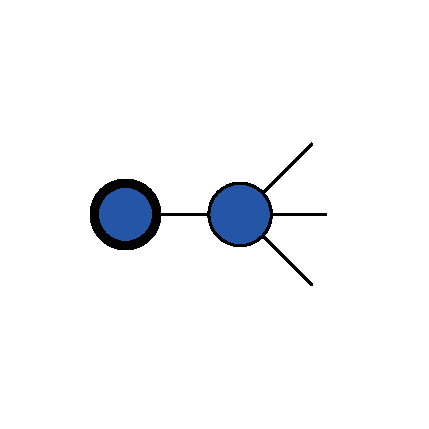
\includegraphics[width = .60\linewidth]{figs/1degbus}
    \subcaption{ 次数1の母線}
    \label{fig:N1} 
  \end{minipage}
  \begin{minipage}{0.3\linewidth}
    \centering
    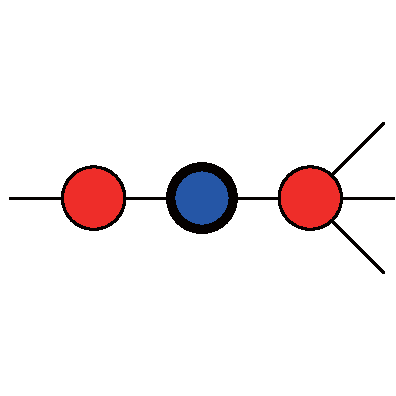
\includegraphics[width = .60\linewidth]{figs/2degbus}
    \subcaption{ 次数2の母線}
  \end{minipage}
  \label{fig:N2}
  \begin{minipage}{0.3\linewidth}
    \centering
    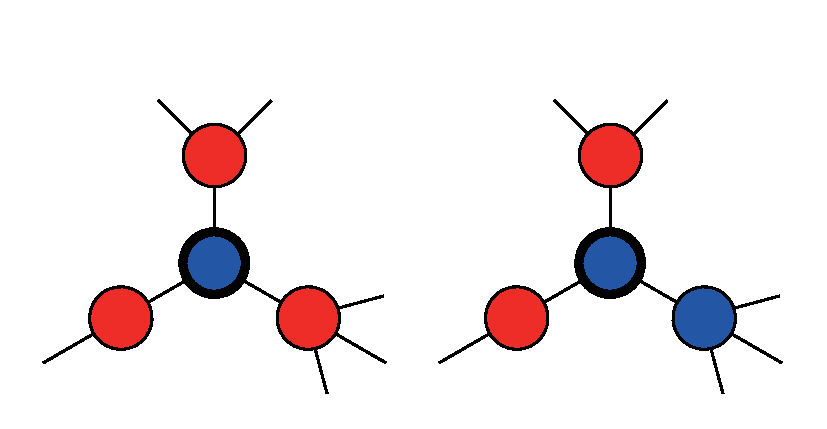
\includegraphics[width = .60\linewidth]{figs/3degbus}
    \subcaption{ 次数3の母線 }
  \end{minipage}
  \medskip
  \caption{母線の次数に応じた隣接母線との同期}
  \label{fig:bussync}
  }
\medskip
\end{figure}
注目する母線の次数が4以上である場合にも同様の解析を行うことは可能である。
しかしながら,得られる条件が$\Omega_i$や$\Omega_j$に関する高次の方程式になることや,任意に選ばれた一部の隣接母線のみが同期する場合などの複数の組み合わせが存在するため,同期に関する等価条件を書き下すことは一般に煩雑となる。
ただし,注目する母線$i$とそれに隣接する$|\mathcal{N}_i|$個の母線に対して,いずれかの$|\mathcal{N}_i |-1$個の隣接母線が母線$i$と同期するのであれば,残り1個の隣接母線も同期することは一般に示される。

補題\ref{lem:sumc2}で示されている次数が3以下の条件を組み合わせて用いることによって,次数が4以上の母線が送電網に含まれている場合にも,すべての母線の同期が示される場合は存在する。
例えば,つぎの事実を示すことができる。

\begin{定理}[木構造の送電網における母線の同期]
\label{thm:tree}
式\ref{eq:PQVgen}の連立方程式によって機器群が結合された電力系統モデルを考える。
送電網のグラフが木構造をもつとき
\footnote{
グラフ理論において,連結であり閉路をもたないグラフは\emph{木}(tree)と呼ばれる。
},定常潮流状態においてすべての母線は同期する。
\end{定理}

\begin{証明}
\FIGref{fig:treepr}(a)の太線で示された端点の母線に注目する。
母線の次数は1であるから,その隣の母線は端点の母線と同期する。
つぎに,端点の隣の母線が鎖状経路にある場合には,その母線の次数は2であるため,少なくともその両隣の母線は同期する。
これを繰り返していくことで,\FIGref{fig:treepr}(a)のように,端点と次数が3以上の節の母線を結ぶ鎖状経路において,すべての母線の同期が示される。

同様に,別の端点から次数が3以上の節に存在するすべての母線は同期するため,\FIGref{fig:treepr}のように,太線で示される節の母線に連結するすべての鎖状経路の母線はすべて同期することがわかる。
この議論を繰り返せば,木を構成するすべての母線が同期することが示される。
\end{証明}


\begin{figure}[t]
  \centering
  {
  \begin{minipage}{0.40\linewidth}
    \centering
    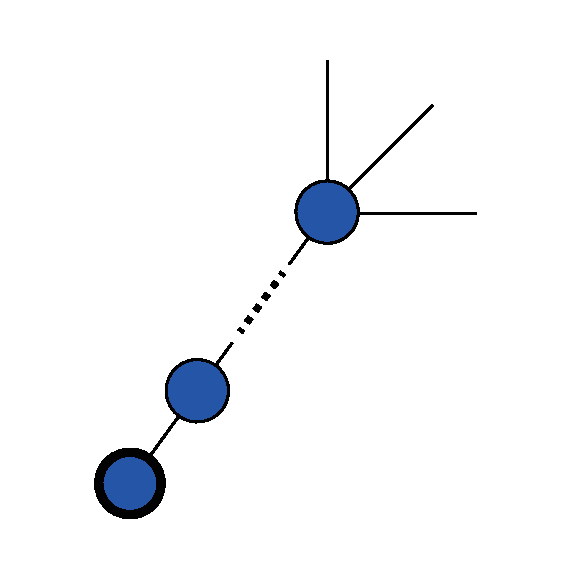
\includegraphics[width = .50\linewidth]{figs/treesub}
    \subcaption{ }
  \end{minipage}
  \begin{minipage}{0.40\linewidth}
    \centering
    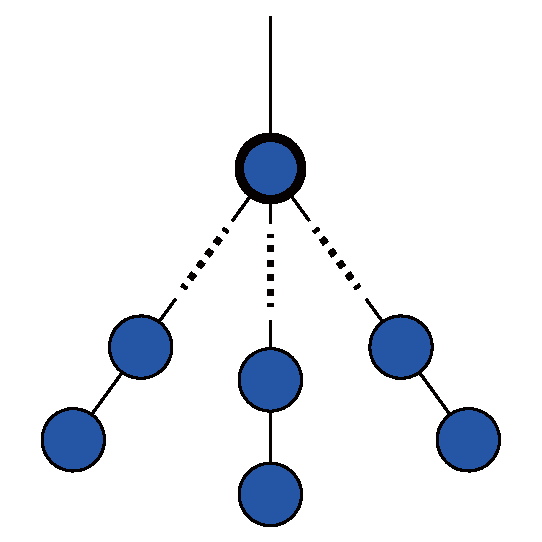
\includegraphics[width = .50\linewidth]{figs/tree}
    \subcaption{ }
  \end{minipage}
  \medskip
  \caption{木構造をもつ送電網における母線の同期}
  \label{fig:treepr}
  }
\medskip
\end{figure}
%\begin{figure}[t]
%\centering
%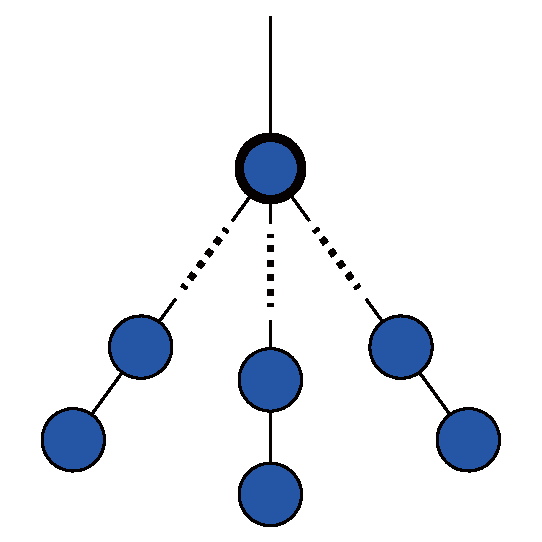
\includegraphics[width = .20\linewidth]{figs/tree}
%\caption{...}
%\label{fig:treepr}
%\medskip
%\end{figure}
定理\ref{thm:tree}に示されている木構造をもつ送電網の母線には次数の制限はない。
このように,仮に次数が4以上の母線が送電網に含まれていたとしても,グラフ構造の情報だけを用いて,すべての母線の同期を演繹できる場合がある。
同様に,つぎの事実を示すことができる。

\begin{定理}[円環構造の送電網における母線の同期]
\label{thm:circ}
式\ref{eq:PQVgen}の連立方程式によって機器群が結合された電力系統モデルを考える。
送電網のグラフが円環構造をもち,かつ,母線の総数が奇数であるとき,定常潮流状態においてすべての母線は同期する。
\end{定理}

\begin{証明}
ある母線に注目するとその両端の母線の同期が示される。
これを繰り返すことにより,母線の総数が奇数である場合にすべての母線の同期が示される。
\end{証明}

\begin{figure}[t]
  \centering
  {
  \begin{minipage}{0.3\linewidth}
    \centering
    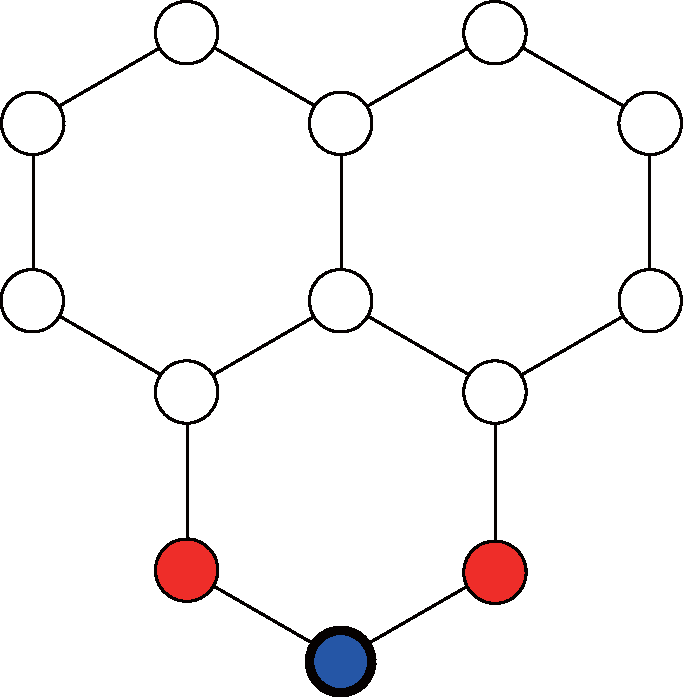
\includegraphics[width = .70\linewidth]{figs/honya}
    \subcaption{  }
  \end{minipage}
  \begin{minipage}{0.3\linewidth}
    \centering
    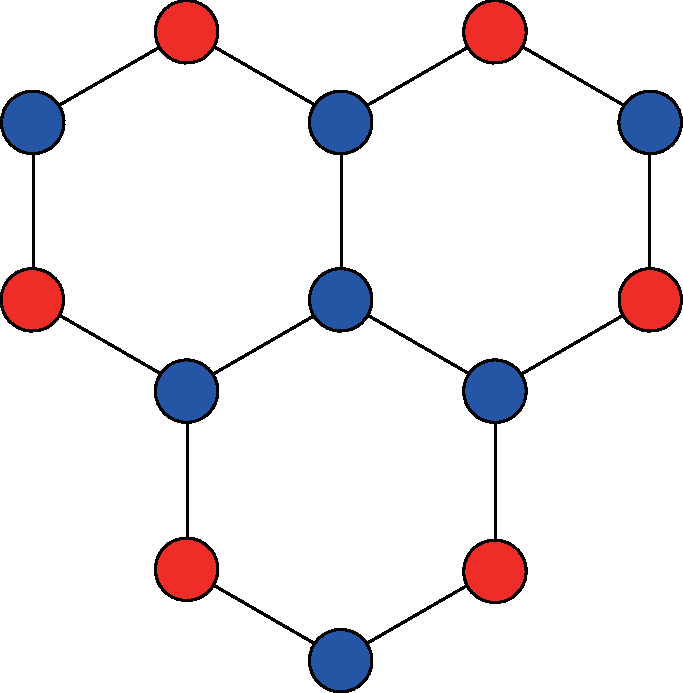
\includegraphics[width = .70\linewidth]{figs/honyb}
    \subcaption{  }
  \end{minipage}
  \begin{minipage}{0.3\linewidth}
    \centering
    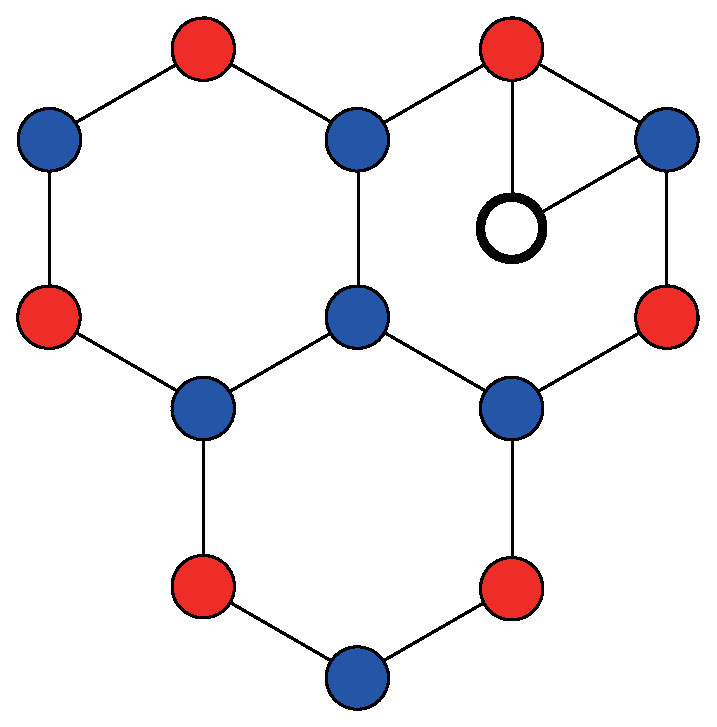
\includegraphics[width = .70\linewidth]{figs/honyc}
    \subcaption{  }
  \end{minipage}
  \medskip
  \caption{ハニカム構造をもつ送電網における母線の同期}
  \label{fig:hony}
  }
\medskip
\end{figure}
定理\ref{thm:circ}は,円環構造の送電網に対して,母線の総数が奇数である場合は,各送電網のアドミタンスの値などに依らず,すべての母線が同期することを示している。
一方で,母線の総数が偶数である場合には,送電線のアドミタンス値などの追加の情報を用いない限りは,円環構造の送電網に対してもすべての母線の同期を結論づけることはできない。
後述する例\ref{ex:symbox}では,母線の総数が偶数である場合にも,アドミタンスの値などの一部の情報が与えられるだけで,すべての母線の同期が示され得ることを示す。
次数3の母線を含む送電網に補題\ref{lem:sumc2}を適用した例としてつぎを示す。

\begin{例}[ハニカム構造の送電網における母線の同期]\label{ex:deg3}
\FIGref{fig:hony}(a)に示されるハニカム構造をもつ送電網に対して,定常潮流状態における母線の同期を考えよう。
最下部の母線に注目すると,その両隣の母線の同期がわかる。
これらの同期する母線を赤で示し,最下部の母線と同期するものを青で示す。
このとき,補題\ref{lem:sumc2}を各母線に適用していくことによって,同期するすべての母線群を\FIGref{fig:hony}(b)のように色分けすることができる。
しかしながら,この場合には,グラフ構造の情報だけで赤の母線群と青の母線群の同期を結論づけることはできない。
一方で,\FIGref{fig:hony}(c)のように母線が1つ追加された送電網の場合には,その追加された母線に注目することで,両隣の赤と青の母線の同期が導かれる。
したがって,\FIGref{fig:hony}(c)のグラフ構造の場合には,すべての母線の同期が示される。
\end{例}

例\ref{ex:deg3}において,一部のグラフ構造の差異により同期する母線の対称性が崩れることで,電力系統全体での母線の同期が演繹されている点は興味深い。
つぎの例では,アドミタンスの値まで考慮した「定量的な送電網の対称性」の観点から母線の同期を考察する。

\begin{figure}[t]
\centering
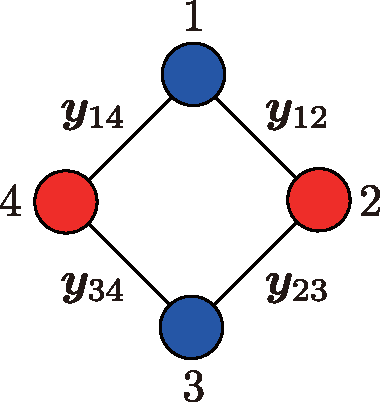
\includegraphics[width = .20\linewidth]{figs/4busbox}
\medskip
\caption{円環構造をもつ送電網における4母線の同期}
\label{fig:4busbox}
\medskip
\end{figure}

\begin{例}[円環構造の送電網における4つの母線の同期]\label{ex:symbox}
\FIGref{fig:4busbox}に示される円環構造をもつ送電網に対して,定常潮流状態における母線の同期を考えよう。
母線の数は偶数であるため,定理\ref{thm:circ}のようにグラフ構造の情報だけですべての母線の同期を示すことはできない。
ただし,\FIGref{fig:4busbox}の赤と青で示されているように,少なくとも互い違いの母線がそれぞれ同期することは補題\ref{lem:sumc2}からわかる。
したがって,すべての母線の同期を示すためには,少なくとも1つの母線に対して式\ref{eq:N2sing}のいずれかの条件が満たされないことを示せば良い。

母線$i$と母線$j$を結ぶ送電線のアドミタンスを$\bm{y}_{ij}$と表す。
このとき,各母線に対する式\ref{eq:N2sing}中央の条件は
\begin{align*}
|\bm{V}_2^{\star}||\bm{y}_{12}|&=|\bm{V}_4^{\star}||\bm{y}_{14}|
,\qquad
|\bm{V}_1^{\star}||\bm{y}_{12}|=|\bm{V}_3^{\star}||\bm{y}_{23}|,
\\
|\bm{V}_2^{\star}||\bm{y}_{23}|&=|\bm{V}_4^{\star}||\bm{y}_{34}|
,\qquad
|\bm{V}_3^{\star}||\bm{y}_{34}|=|\bm{V}_1^{\star}||\bm{y}_{14}|
\end{align*}
と書き下すことができる。
これを行列形式で表現すれば
\begin{align*}
\underbrace{
\mat{
0 & |\bm{y}_{12}| &  0  & -|\bm{y}_{14}|\\
-|\bm{y}_{12}| & 0 & |\bm{y}_{23}| & 0\\
0 & -|\bm{y}_{23}| & 0 & |\bm{y}_{34}|\\
|\bm{y}_{14}| & 0 & -|\bm{y}_{34}| & 0
}}_{S}
\mat{
|\bm{V}_1^{\star}|\\
|\bm{V}_2^{\star}|\\
|\bm{V}_3^{\star}|\\
|\bm{V}_4^{\star}|
}=0
\end{align*}
となる。
この方程式を満たす正のベクトル$(|\bm{V}_1^{\star}|,\ldots,|\bm{V}_4^{\star}|)$が存在するための必要条件は,左辺の$S$が正則でないことである。
%ただし,$S$が正則でない場合にも,正のベクトルがその零空間として存在するとは限らないことに注意されたい。
ここで,列ベクトルの疎構造から,$S$が非正則であるためには
\begin{align}\label{eq:ycond}
|\bm{y}_{12}||\bm{y}_{34}| = |\bm{y}_{14}||\bm{y}_{23}|
\end{align}
でなければならない。
したがって,アドミタンス行列がこの条件を満たさない限り,すべての母線は同期する。
なお,式\ref{eq:ycond}が満たされる場合には,所望の電圧フェーザの絶対値を定めることができるため,式\ref{eq:N2sing}中央の条件を満たす$(|\bm{V}_1^{\star}|,\ldots,|\bm{V}_4^{\star}|)$が存在するための必要十分条件が,式\ref{eq:ycond}であることも示される。

つぎに,式\ref{eq:N2sing}右の条件は,母線1と母線3に注目すれば
\begin{align*}
|\phi_2 - \phi_4 + \angle \bm{y}_{12} - \angle \bm{y}_{14}|=\pi
,\qquad
|\phi_2 - \phi_4 + \angle \bm{y}_{23} - \angle \bm{y}_{34}|=\pi
\end{align*}
と書き下すことができる。
同様に,母線2と母線4に注目すれば
\begin{align*}
|\phi_1 - \phi_3 + \angle \bm{y}_{12} - \angle \bm{y}_{23}|=\pi
,\qquad
|\phi_1 - \phi_3 + \angle \bm{y}_{14} - \angle \bm{y}_{34}|=\pi
\end{align*}
が得られる。
一般に,アドミタンスの実部であるコンダクタンス成分は非負であり,虚部であるサセプタンス成分は負であること,すなわち,
\[
\angle \bm{y}_{ij} \in \left[-\frac{\pi}{2},0 \right)
\]
であることに注意すると,以上の条件を満たす$(\phi_1,\ldots,\phi_4)$が存在するための必要十分条件が
\begin{align}\label{eq:ycona}
\angle \bm{y}_{12} - \angle \bm{y}_{14}=
\angle \bm{y}_{23} - \angle \bm{y}_{34}
\end{align}
であることが導ける。
したがって,アドミタンス行列がこの条件を満たさない限り,すべての母線は同期する。

以上の議論から,定常潮流状態において同期しない母線の組が1つ以上存在するための必要十分条件は,式\ref{eq:ycond}かつ式\ref{eq:ycona}であることがわかる。
この2つの条件は,\FIGref{fig:4busbox}の送電網がアドミタンスの値に関する特異的な対称性をもつときにのみ,互い違いの母線のみが同期するような状況が起こることを示唆している。
\end{例}

例\ref{ex:symbox}から,式\ref{eq:N2sing}の条件は送電網のアドミタンスの値に関する特異的な対称性を表すことがわかる。
実応用においては,各母線の次数が高くない疎な送電網に対してすべての母線が定常潮流状態で同期することは,そのグラフ構造に特異的な対称性が存在しない限りは普遍的な事実である。
実際,著者らが知る限りにおいて,現実的な値に設定されたいかなる電力系統モデルのパラメータに対しても,定常潮流状態におけるすべての母線の同期が数値的に確かめられている。

%\red{(以下、不要かも)}
%
%さいごに,以上の議論から導かれるつぎの事実を示す。
%
%\begin{定理}[母線変数の計測による母線同期の判定]
%\label{cor:PQsync}
%式\ref{eq:PQVgen}の連立方程式によって機器群が結合された電力系統モデルを考える。
%電力系統は定常潮流状態にあるものと仮定する。
%このとき,次数2の母線$i$に対して
%\begin{align}\label{eq:PQnot2}
%P_i \neq \real[\bm{Y}_{ii}] |\bm{V}_i|^2
%\qquad
%{\rm または}
%\qquad
%Q_i \neq - \imag [\bm{Y}_{ii}] |\bm{V}_i|^2
%\end{align}
%が成り立つ,もしくは,その隣接母線に対して
%\begin{align}\label{eq:VYnot2}
%\spliteq{
%& |\bm{V}_{j_1}| |\bm{Y}_{ij_1}| \neq 
%|\bm{V}_{j_2}| |\bm{Y}_{ij_2}|
%\qquad
%{\rm または} \\
%& |\angle \bm{V}_{j_1} - \angle \bm{V}_{j_2} - \angle \bm{Y}_{ij_1} + \angle \bm{Y}_{ij_2} | \neq \pi
%}
%\end{align}
%が成り立つならば,式\ref{eq:alloms}が成り立つ。
%ただし,$\mathcal{N}_i = \{j_1,j_2\}$である。
%また,次数3の母線$i$に対して,$\Omega_i = \Omega_{j_3}$を満たす$j_3 \in \mathcal{N}_i$が存在するものとする。
%このとき,母線$i$に対して
%\begin{align}\label{eq:PQnot3}
%\spliteq{
% P_i  &\neq \real[\bm{Y}_{ii}] |\bm{V}_i|^2  + |\bm{Y}_{ij_3}| |\bm{V}_i| |\bm{V}_{j_3}| 
%\sfcos (\angle \bm{V}_i - \angle \bm{V}_{j_3} - \angle \bm{Y}_{ij_3}) \\
%& \hspace{6em} {\rm または} 
%\\
%Q_i & \neq - \imag [\bm{Y}_{ii}] |\bm{V}_i|^2  + |\bm{Y}_{ij_3}| |\bm{V}_i| |\bm{V}_{j_3}| 
%\sfsin (\angle \bm{V}_i - \angle \bm{V}_{j_3} - \angle \bm{Y}_{ij_3})
%}
%\end{align}
%が成り立つ,もしくは,その隣接母線に対して式\ref{eq:VYnot2}が成り立つならば,式\ref{eq:alloms}が成り立つ。
%ただし,$ \mathcal{N}_i \setminus \{j_3\}=\{j_1,j_2\}$である。
%\end{定理}
%
%\begin{証明}
%次数2の母線に関する題意を対偶により示す。
%すなわち,式\ref{eq:alloms}の否定,すなわち,式\ref{eq:N2sing}が成り立つならば,式\ref{eq:PQnot2}や式\ref{eq:VYnot2}の否定が成り立つことを示す。
%まず,式\ref{eq:VYnot2}の否定は,式\ref{eq:N2sing}の中央と右そのものであることから,後者の含意は明らかである。
%つぎに,式\ref{eq:N2sing}が成り立つとき,式\ref{eq:sumcirc}の$\bm{c}_i$は0であることが導かれる。
%これは,式\ref{eq:PQnot2}の否定,すなわち
%\begin{align*}
%P_i = \real[\bm{Y}_{ii}] |\bm{V}_i|^2
%,\qquad
%Q_i = - \imag [\bm{Y}_{ii}] |\bm{V}_i|^2
%\end{align*}
%を意味する。
%以上より,次数2の母線に関する題意が示される。
%次数3の母線に関する題意も同様に示される。
%\end{証明}
%
%
%定理\ref{cor:PQsync}により,有効電力や無効電力,電圧フェーザを実際に計測することによって,グラフ構造だけでは判断できなかった母線の同期を示すことが可能となる。
%例えば,\FIGref{fig:hony}(b)のハニカム構造をもつ送電網に対して,定常潮流状態において適当な母線の有効電力や無効電力,電圧フェーザを計測し,いずれかの赤と青の母線の同期を示すことができれば,送電網全体での母線の同期が結論できる。
%


\newpage
\end{document}